%-------------------------------------------------------------------------------
% FIGURE DEFINITIONS WITH CAPTIONS AND LABELS
%-------------------------------------------------------------------------------
% This file contains all figure definitions for consistent formatting

%==============================================================================
% SYSTEM DIAGRAMS (Chapter 3)
%==============================================================================

\newcommand{\figUseCaseDiagram}{%
  \begin{figure}[htbp]
    \centering
    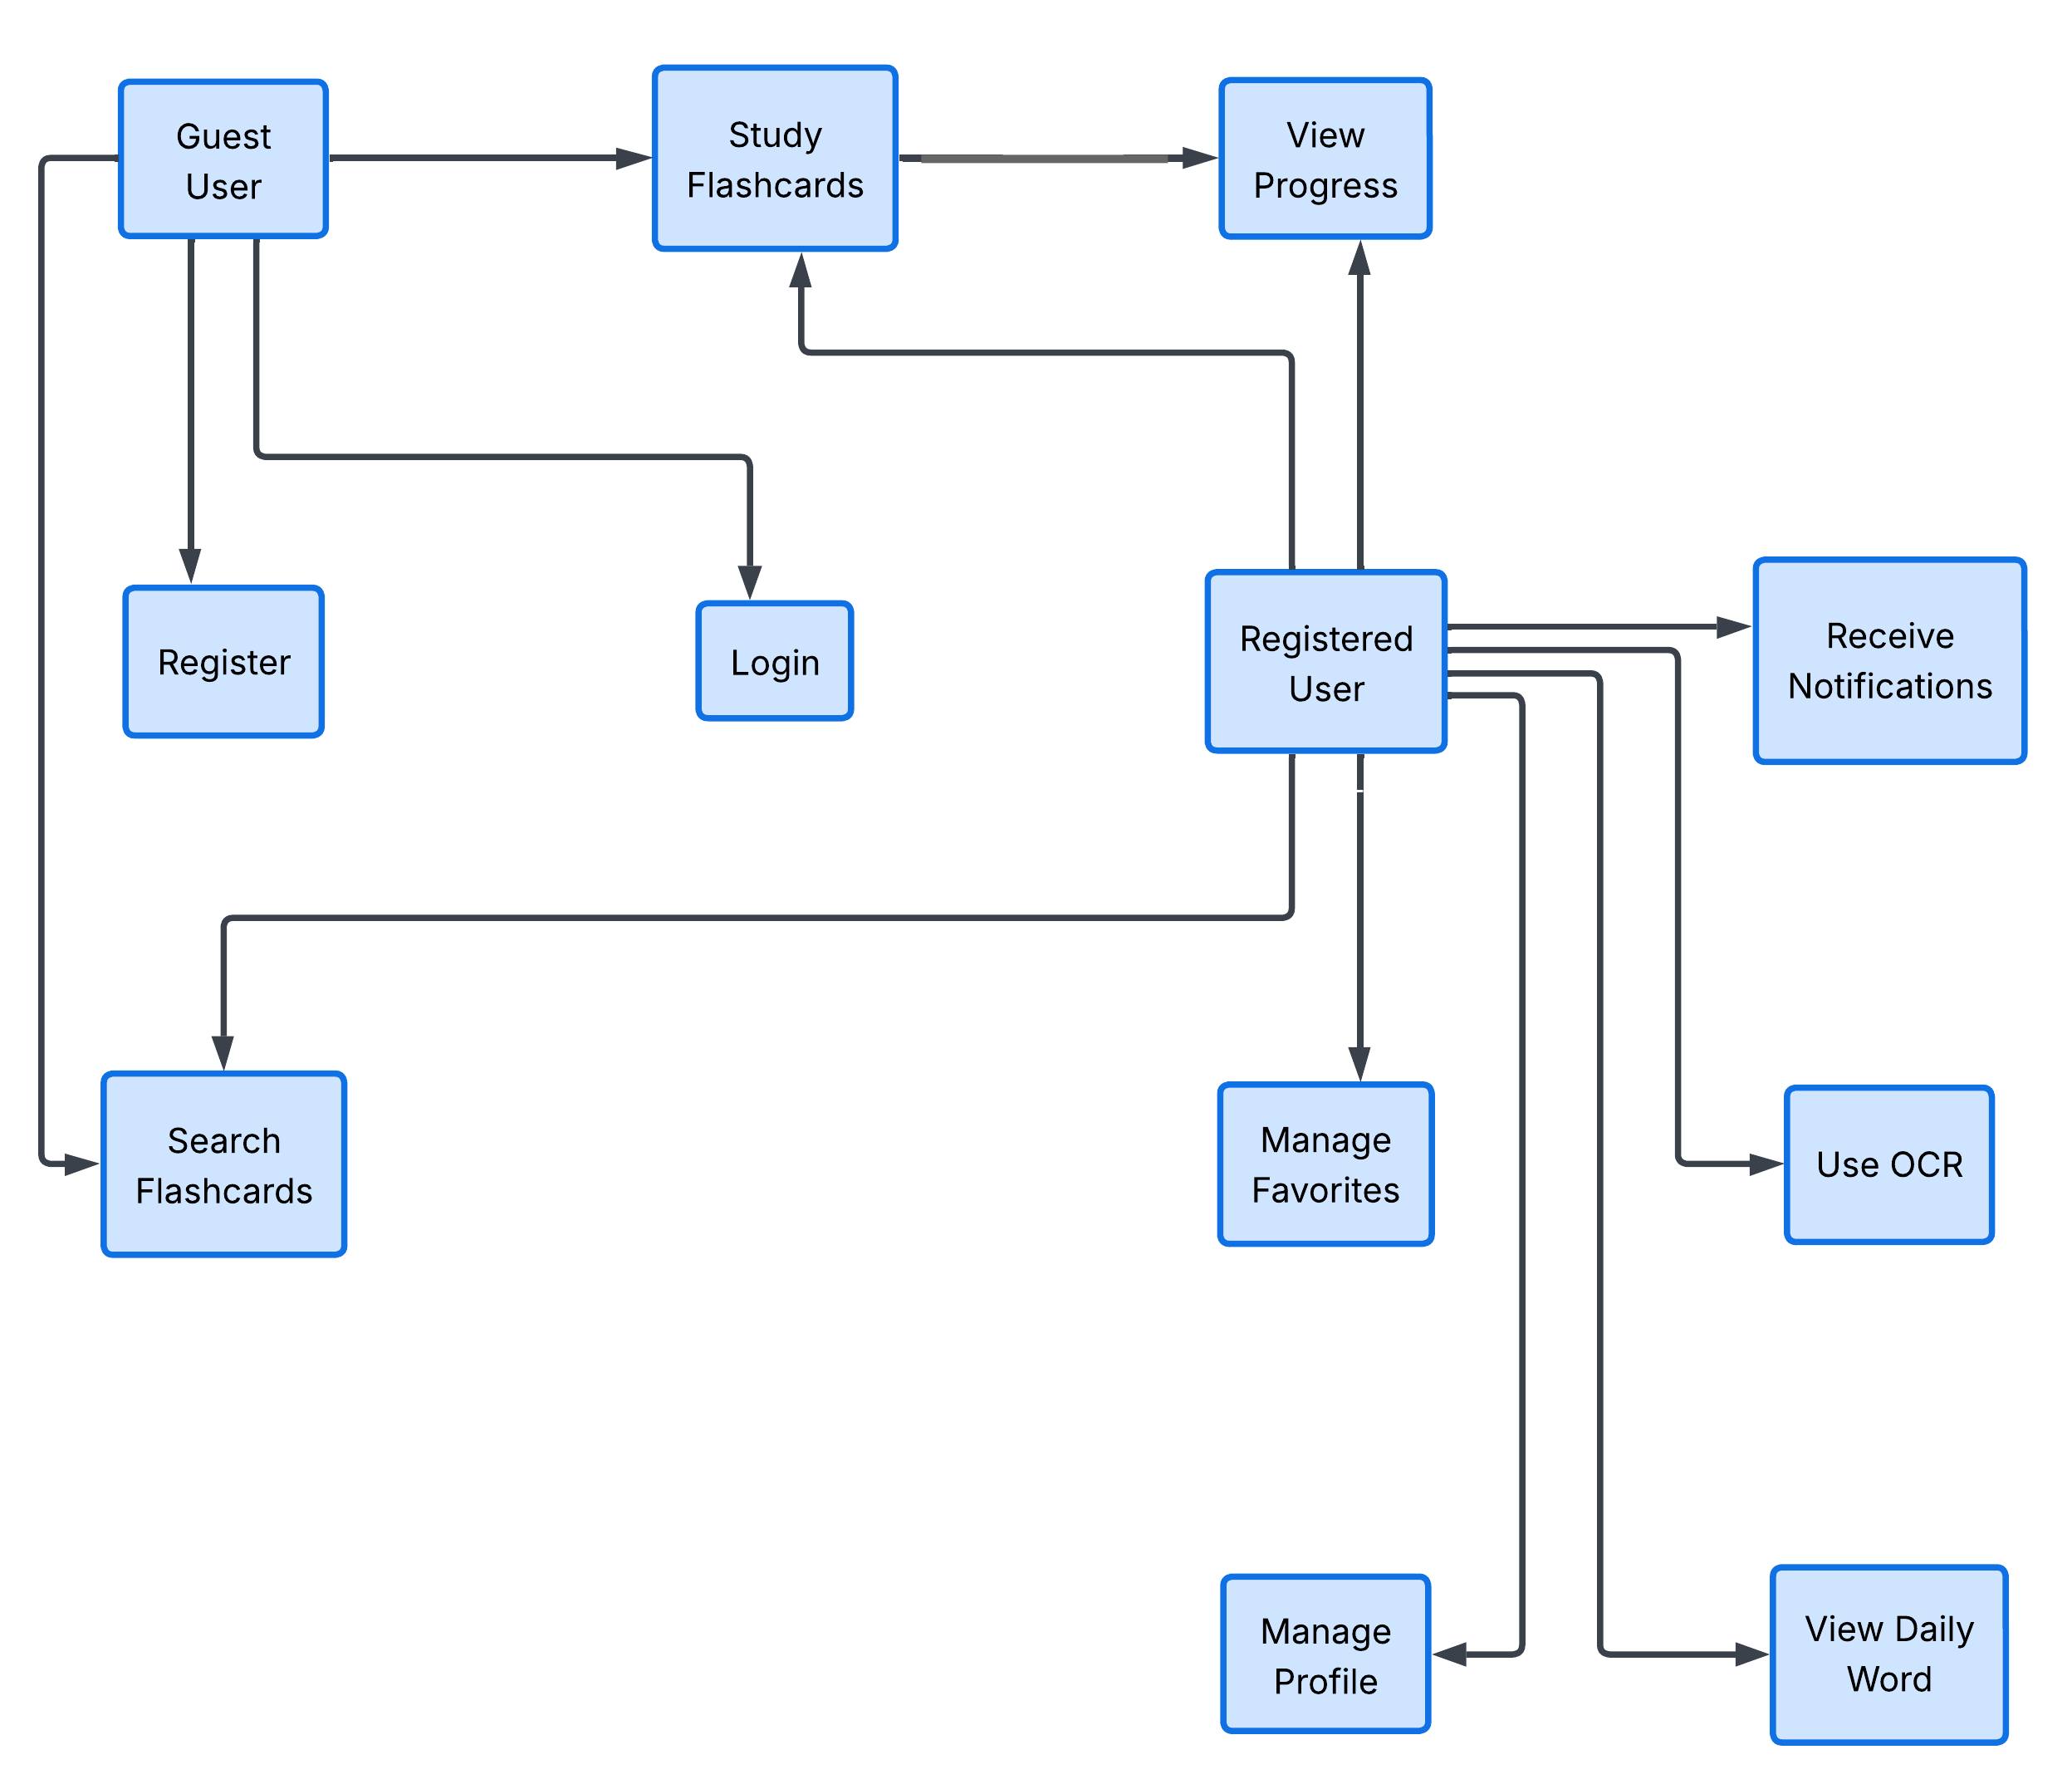
\includegraphics[width=0.8\textwidth]{Figures/diagrams/usecasediagram.png}
    \caption{Egüü системийн үндсэн use case диаграмм.}
    \label{fig:usecase}
  \end{figure}
}

\newcommand{\figSequenceDiagram}{%
  \begin{figure}[htbp]
    \centering
    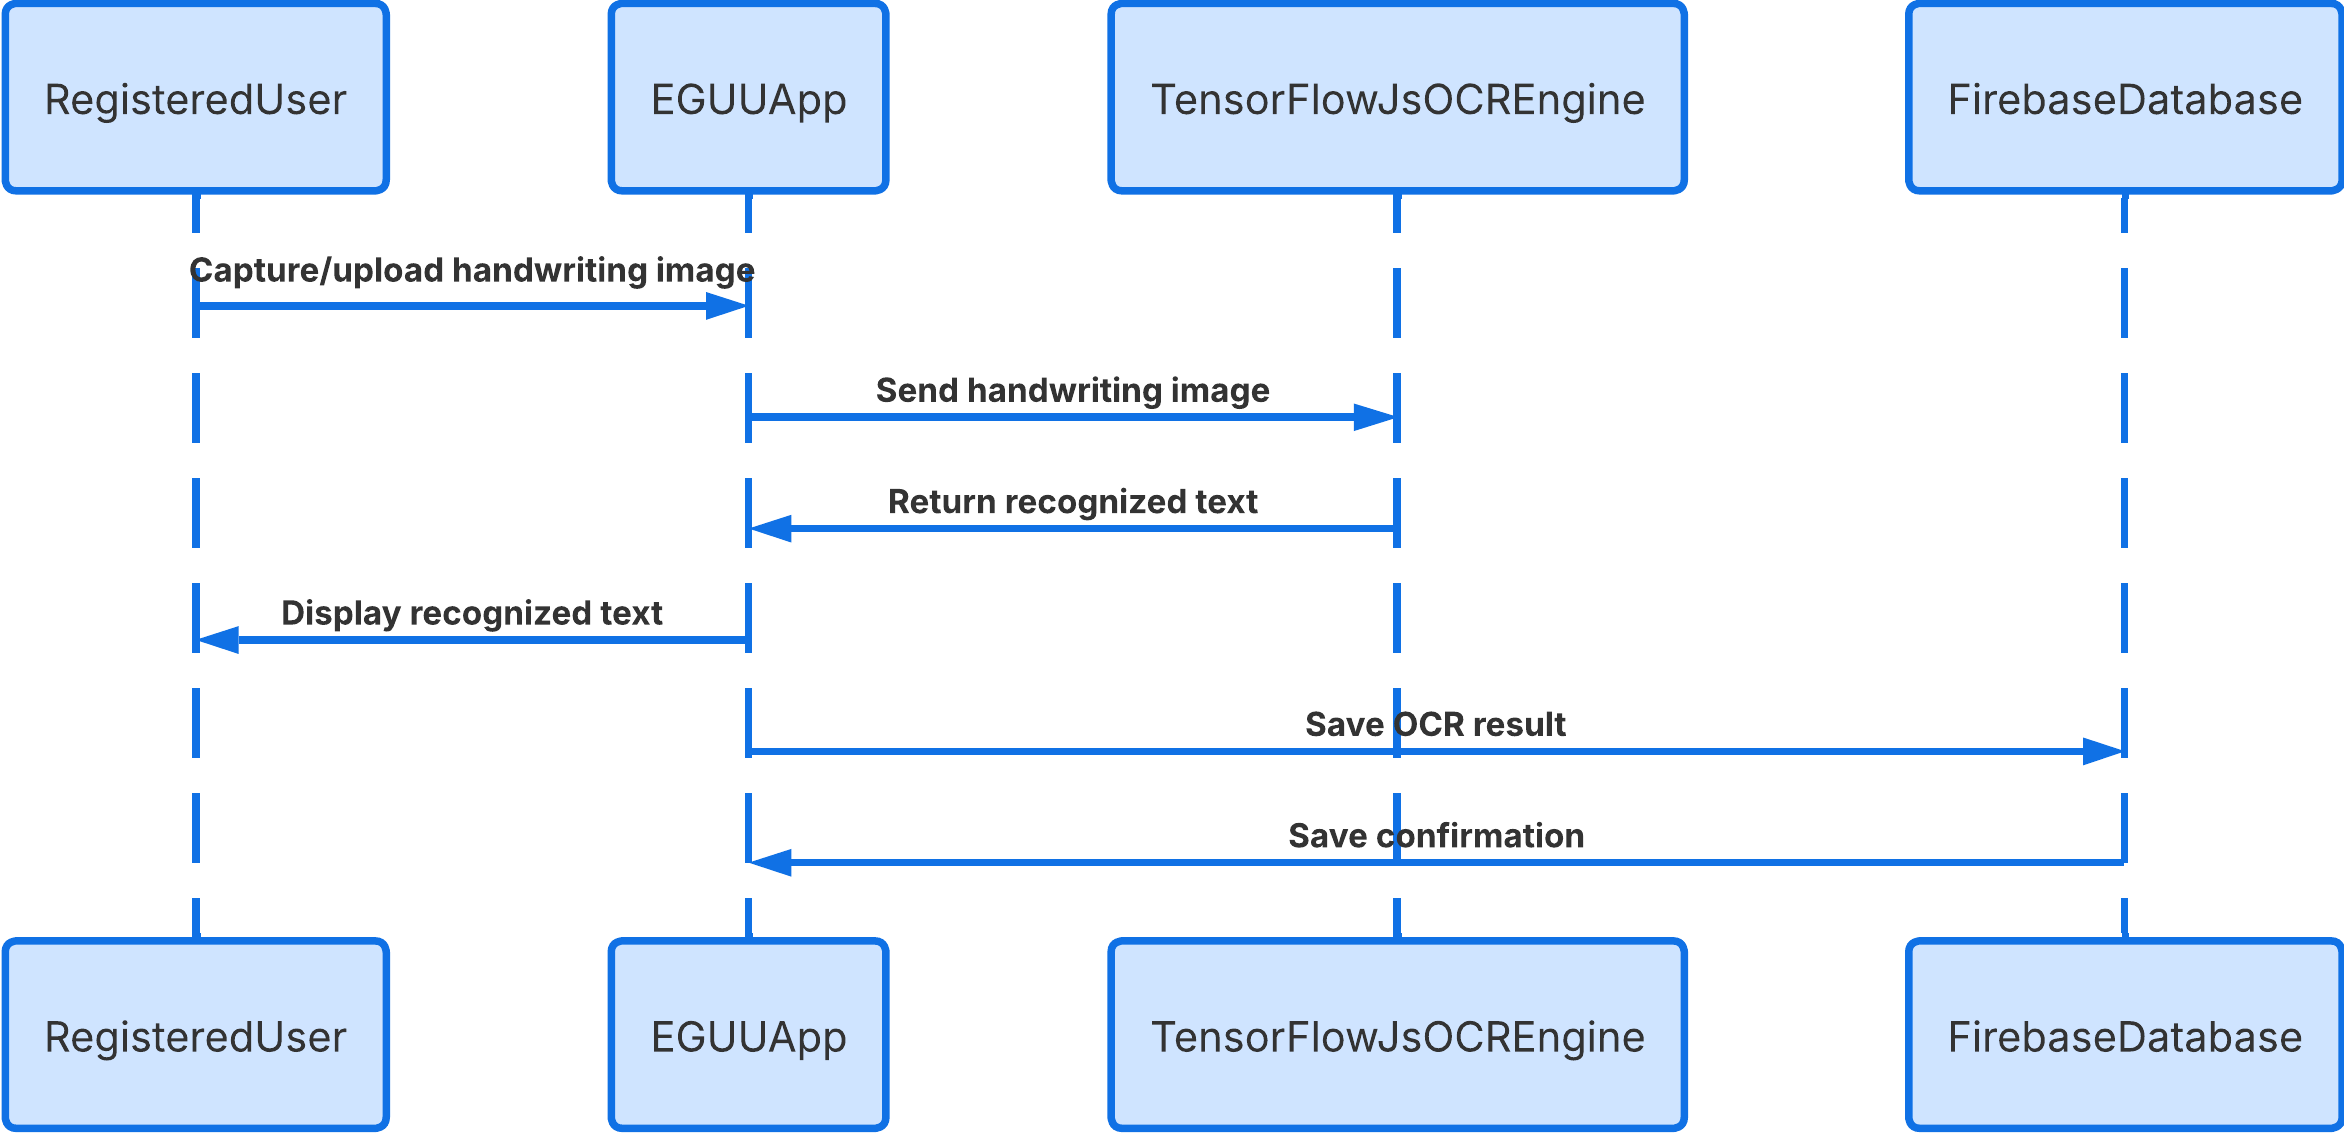
\includegraphics[width=0.85\textwidth]{Figures/diagrams/sequence.png}
    \caption{Хэрэглэгч нэвтрэх үеийн sequence диаграмм.}
    \label{fig:sequence}
  \end{figure}
}

\newcommand{\figERDiagram}{%
  \begin{figure}[htbp]
    \centering
    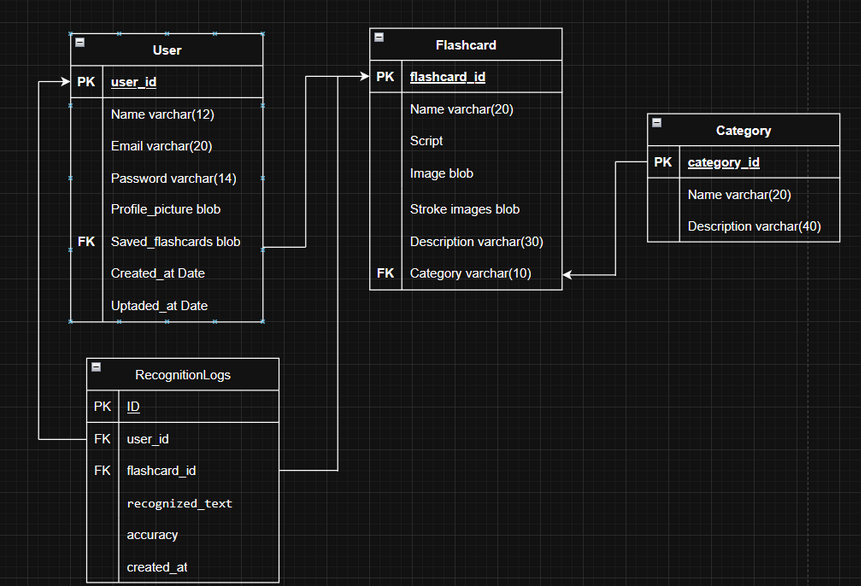
\includegraphics[width=0.8\textwidth]{Figures/diagrams/erd.png}
    \caption{Egüü системийн өгөгдлийн сангийн ER диаграмм.}
    \label{fig:erd}
  \end{figure}
}

\newcommand{\figActivityDiagram}{%
  \begin{figure}[htbp]
    \centering
    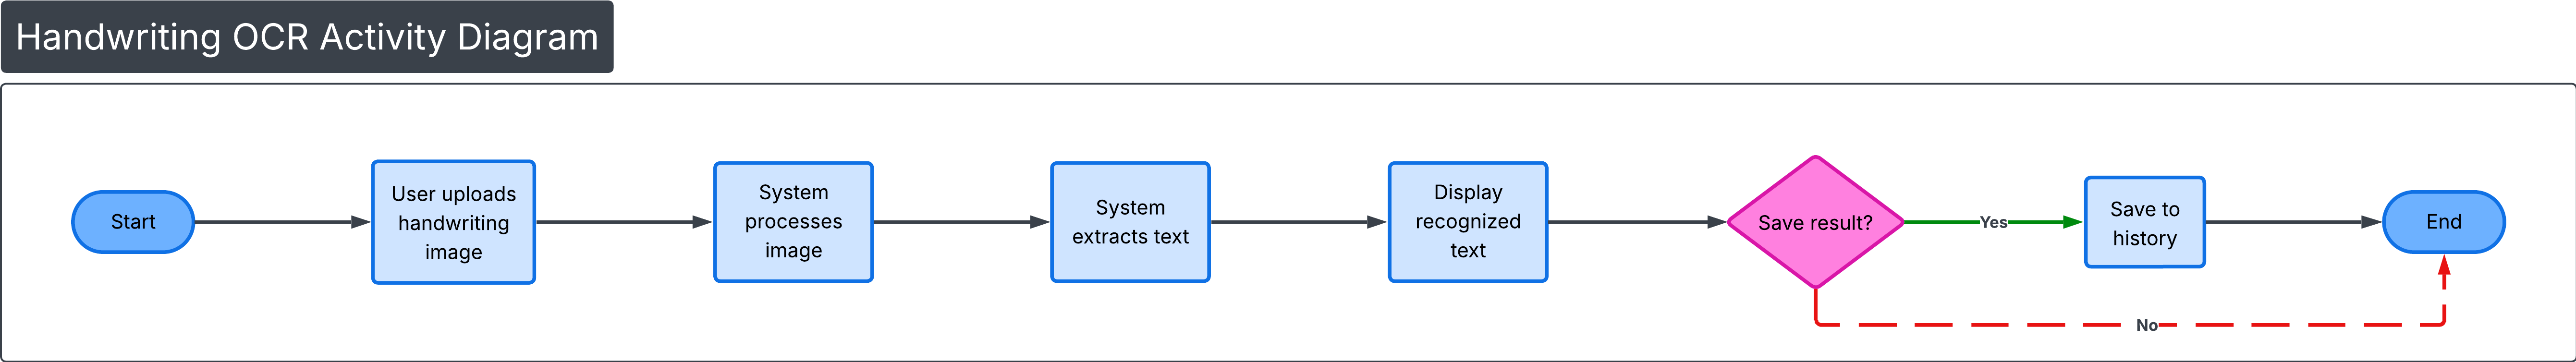
\includegraphics[width=0.8\textwidth]{Figures/diagrams/activitydiagram.png}
    \caption{Flashcard-аар суралцах үйл явцын activity диаграмм.}
    \label{fig:activity}
  \end{figure}
}

\newcommand{\figDataFlowDiagram}{%
  \begin{figure}[htbp]
    \centering
    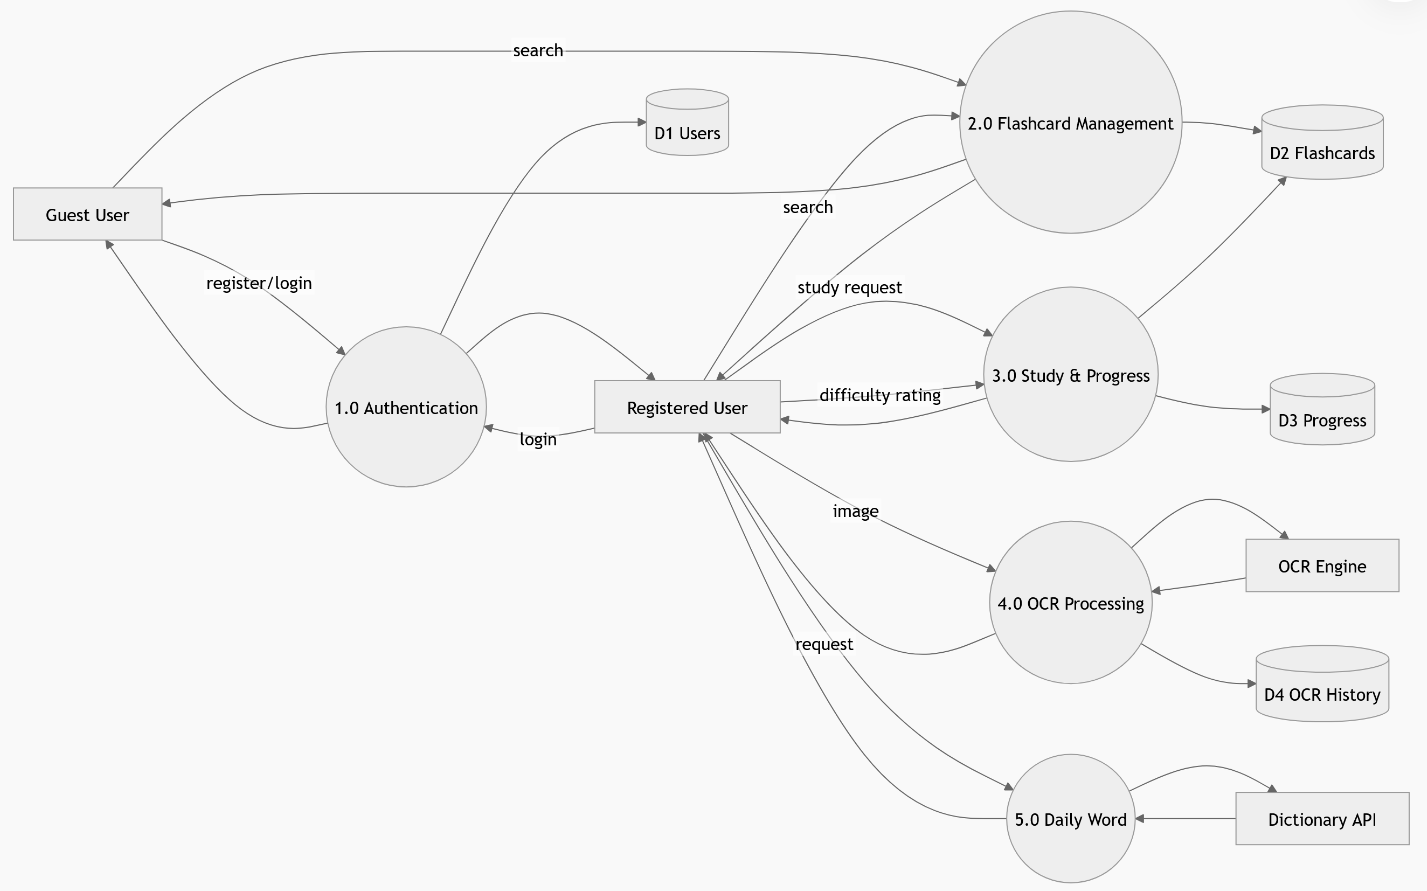
\includegraphics[width=0.85\textwidth]{Figures/diagrams/dataflow.png}
    \caption{Egüü системийн өгөгдөл дамжих урсгалын диаграмм.}
    \label{fig:dataflow}
  \end{figure}
}

%==============================================================================
% FIREBASE ARCHITECTURE (Chapter 4)
%==============================================================================

\newcommand{\figFirebaseAuth}{%
  \begin{figure}[H]
    \centering
    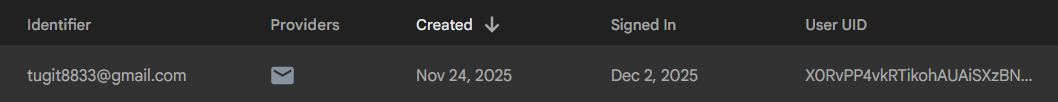
\includegraphics[width=0.75\textwidth]{Figures/firebase/firebaseAuth.png}
    \caption{Firebase Authentication тохиргоо, нэвтрэх аргуудын тохируулга.}
    \label{fig:firebase-auth}
  \end{figure}
}

\newcommand{\figFirebaseDB}{%
  \begin{figure}[H]
    \centering
    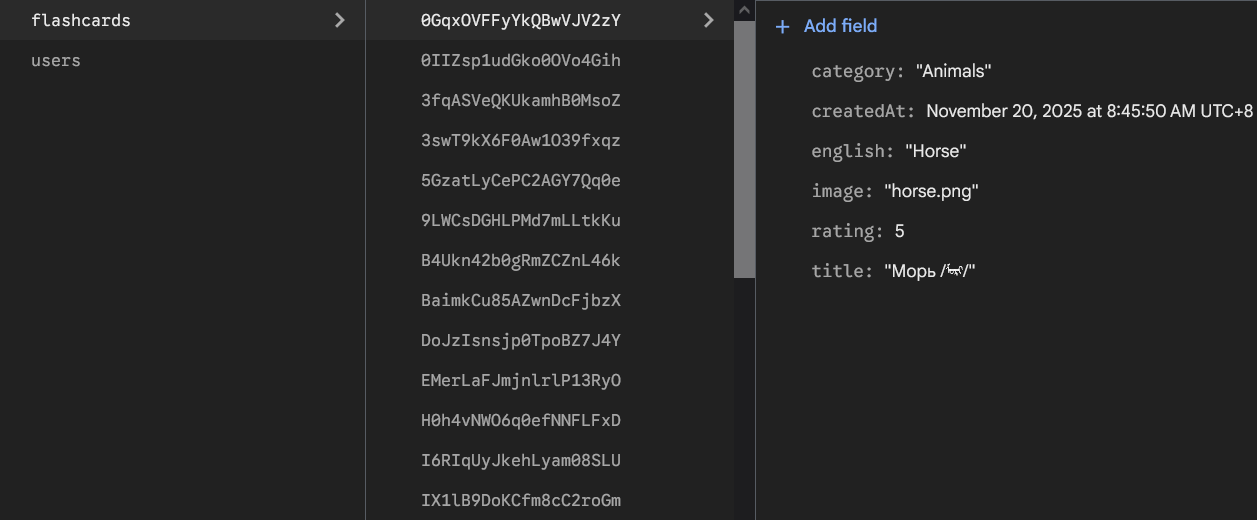
\includegraphics[width=0.8\textwidth]{Figures/firebase/firebaseDB.png}
    \caption{Firestore өгөгдлийн сангийн collection–ийн бүтцийн диаграмм.}
    \label{fig:firebase-db}
  \end{figure}
}

\newcommand{\figFirebaseStorage}{%
  \begin{figure}[H]
    \centering
    
\includegraphics[width=0.75\textwidth]{Figures/firebase/firebaseStorage.png}
    \caption{Firebase Storage дээр зураг, медиа файлууд хадгалах бүтцийн диаграмм.}
    \label{fig:firebase-storage}
  \end{figure}
}

%==============================================================================
% USER INTERFACE - AUTHENTICATION SCREENS (Chapter 4)
%==============================================================================

\newcommand{\figLoginScreen}{%
  \begin{figure}[htbp]
    \centering
    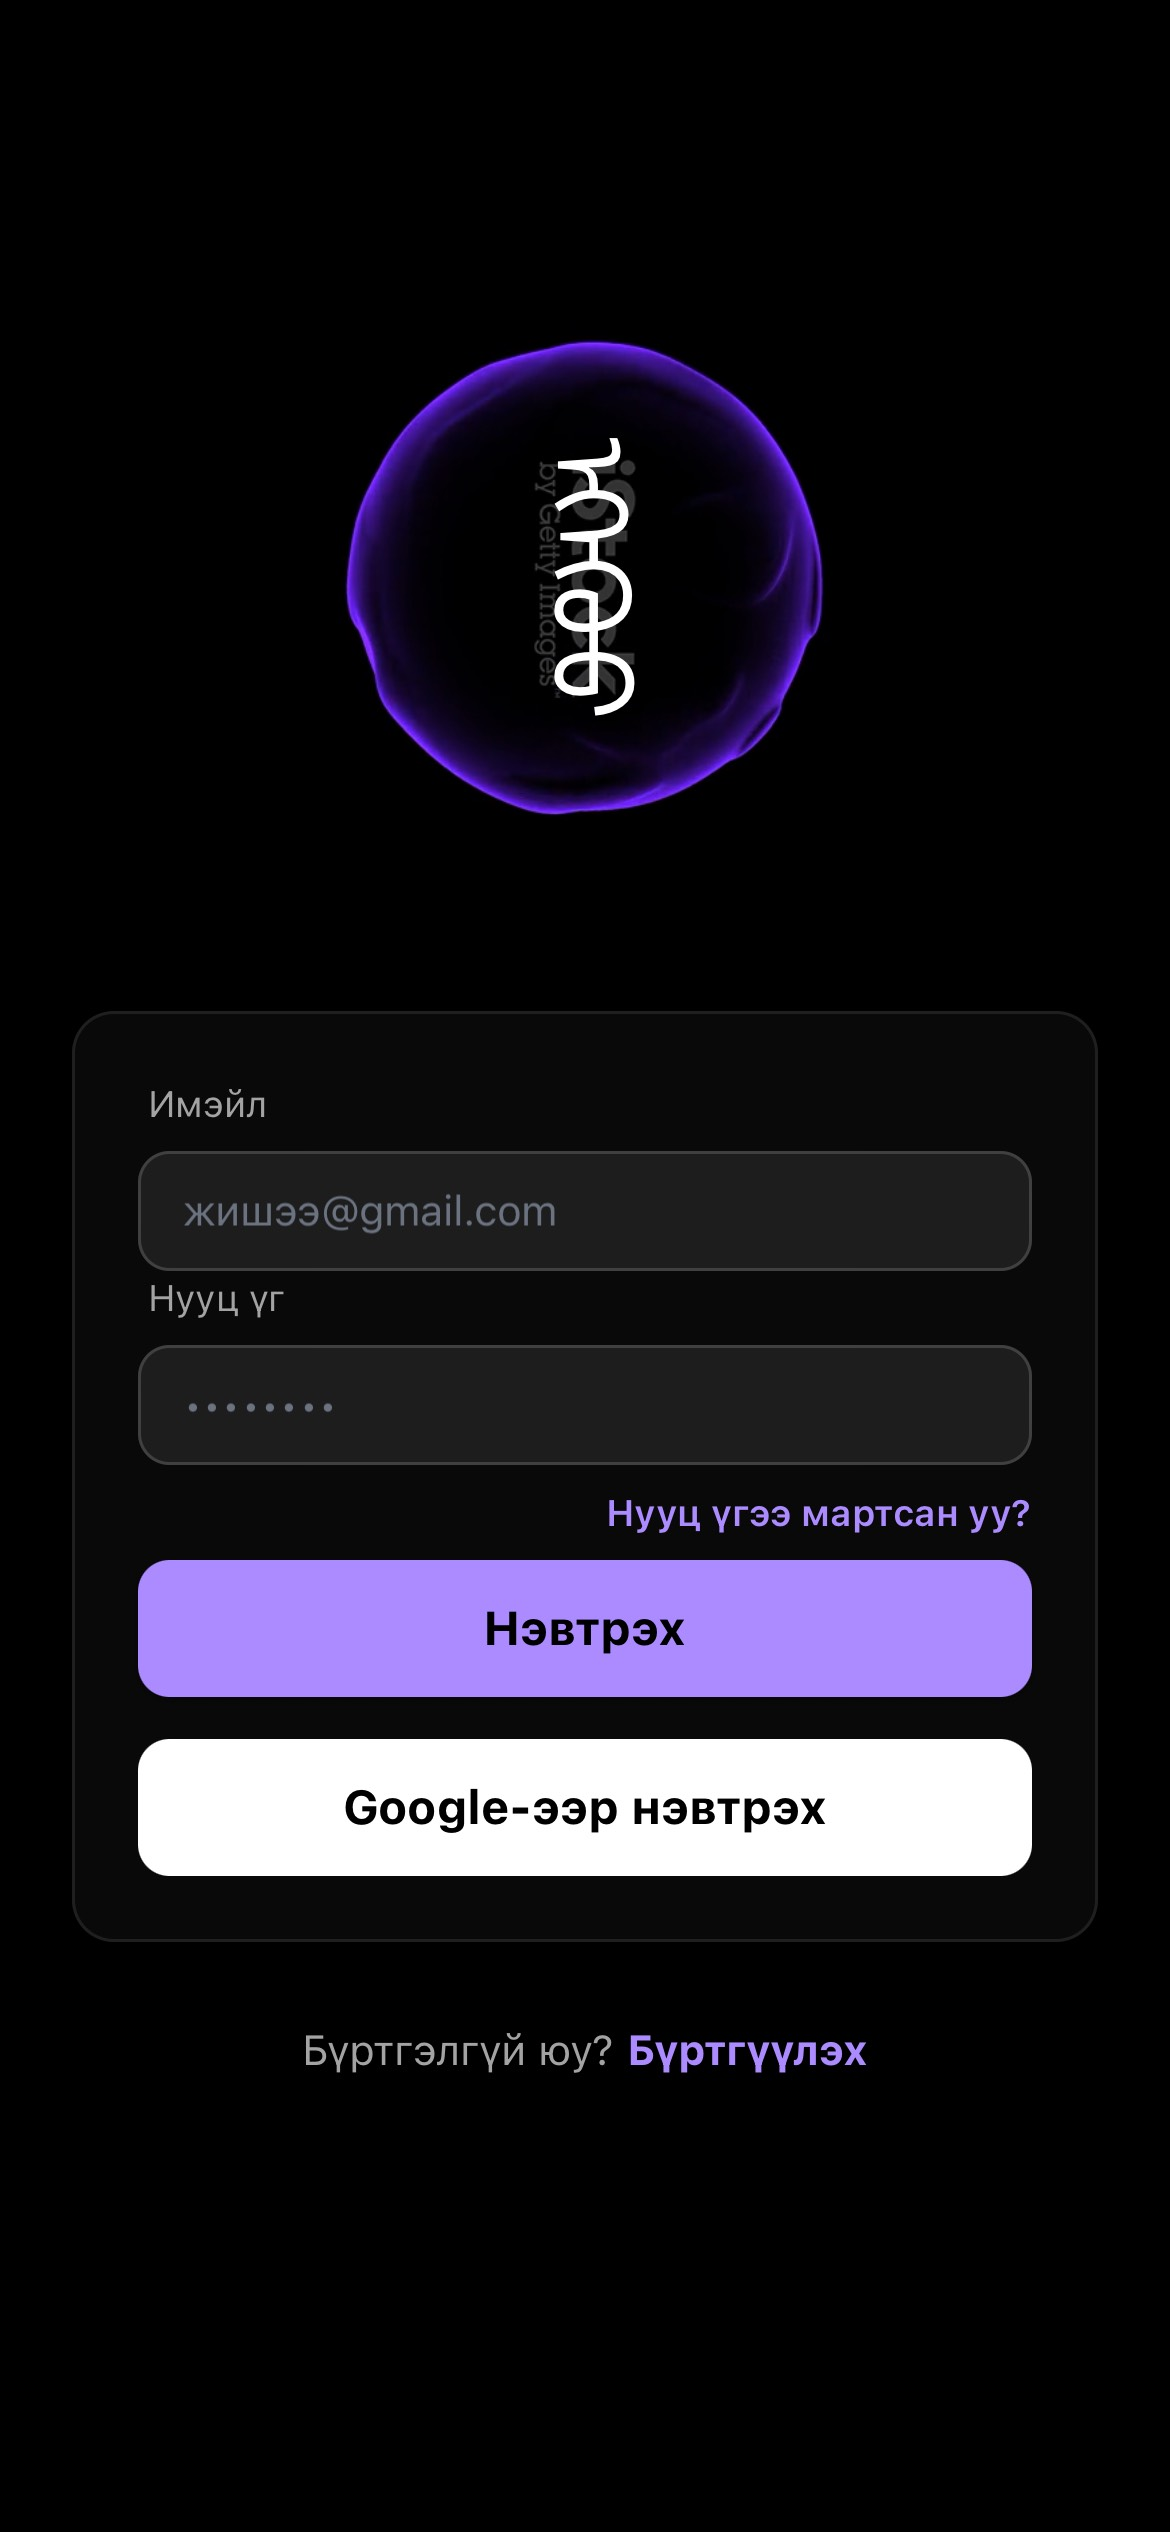
\includegraphics[width=0.35\textwidth]{Figures/pages/Login.png}
    \caption{Нэвтрэх дэлгэц (Email/Password ба Google нэвтрэлт).}
    \label{fig:login}
  \end{figure}
}

\newcommand{\figSignUpScreen}{%
  \begin{figure}[htbp]
    \centering
    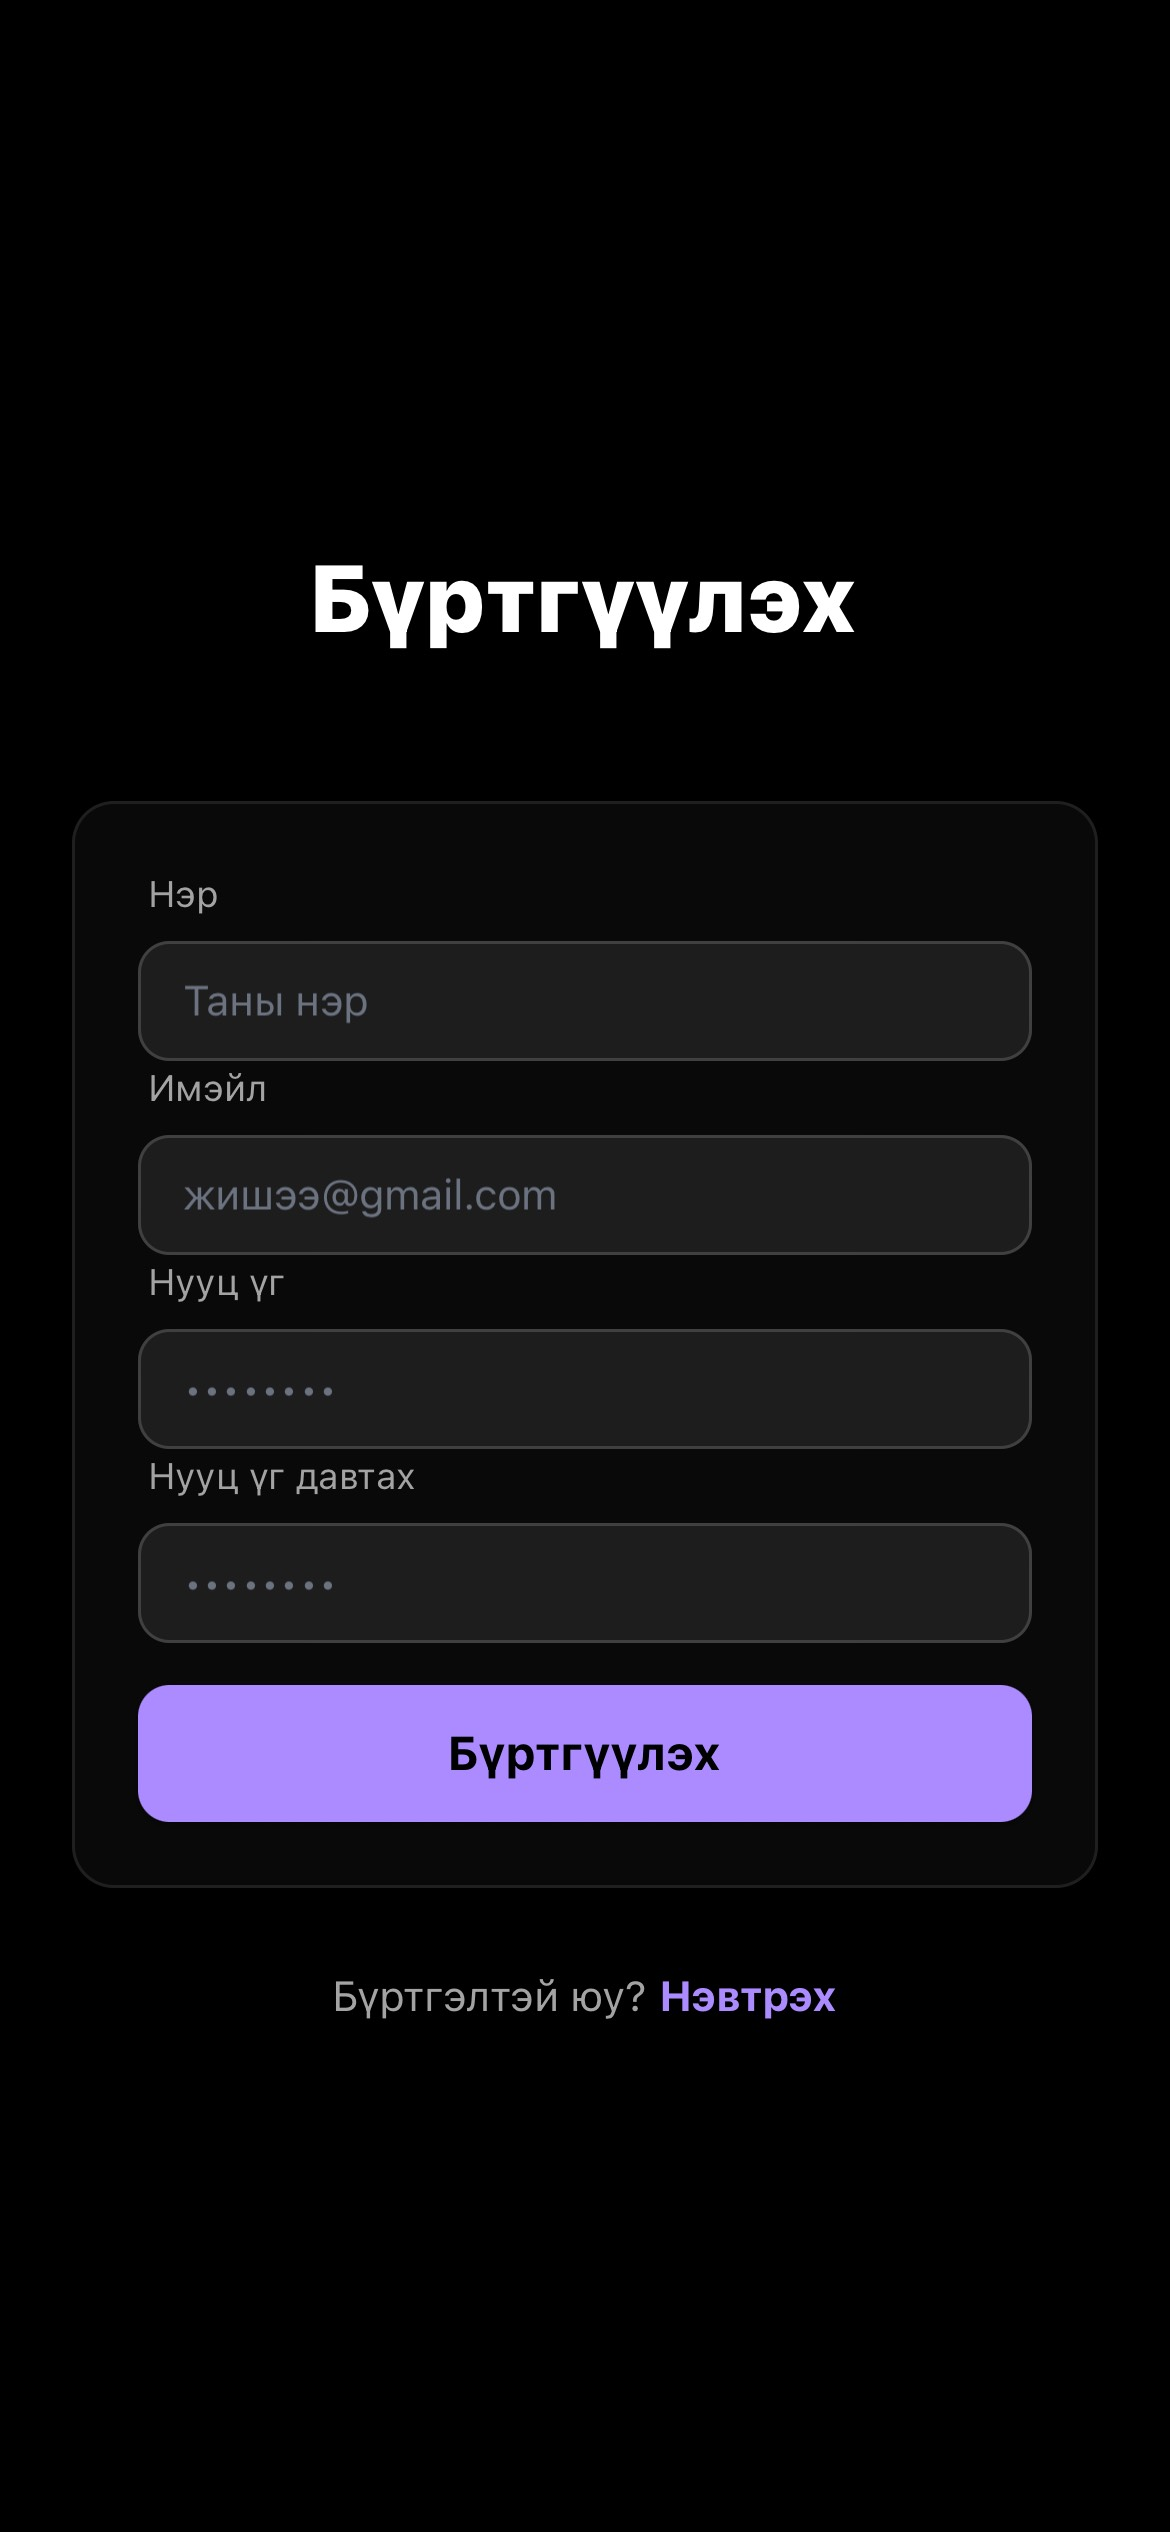
\includegraphics[width=0.35\textwidth]{Figures/pages/SignUp.png}
    \caption{Бүртгүүлэх дэлгэц (шинэ хэрэглэгчийн бүртгэл).}
    \label{fig:signup}
  \end{figure}
}

%==============================================================================
% USER INTERFACE - MAIN SCREENS (Chapter 4)
%==============================================================================

\newcommand{\figHomeScreen}{%
  \begin{figure}[htbp]
    \centering
    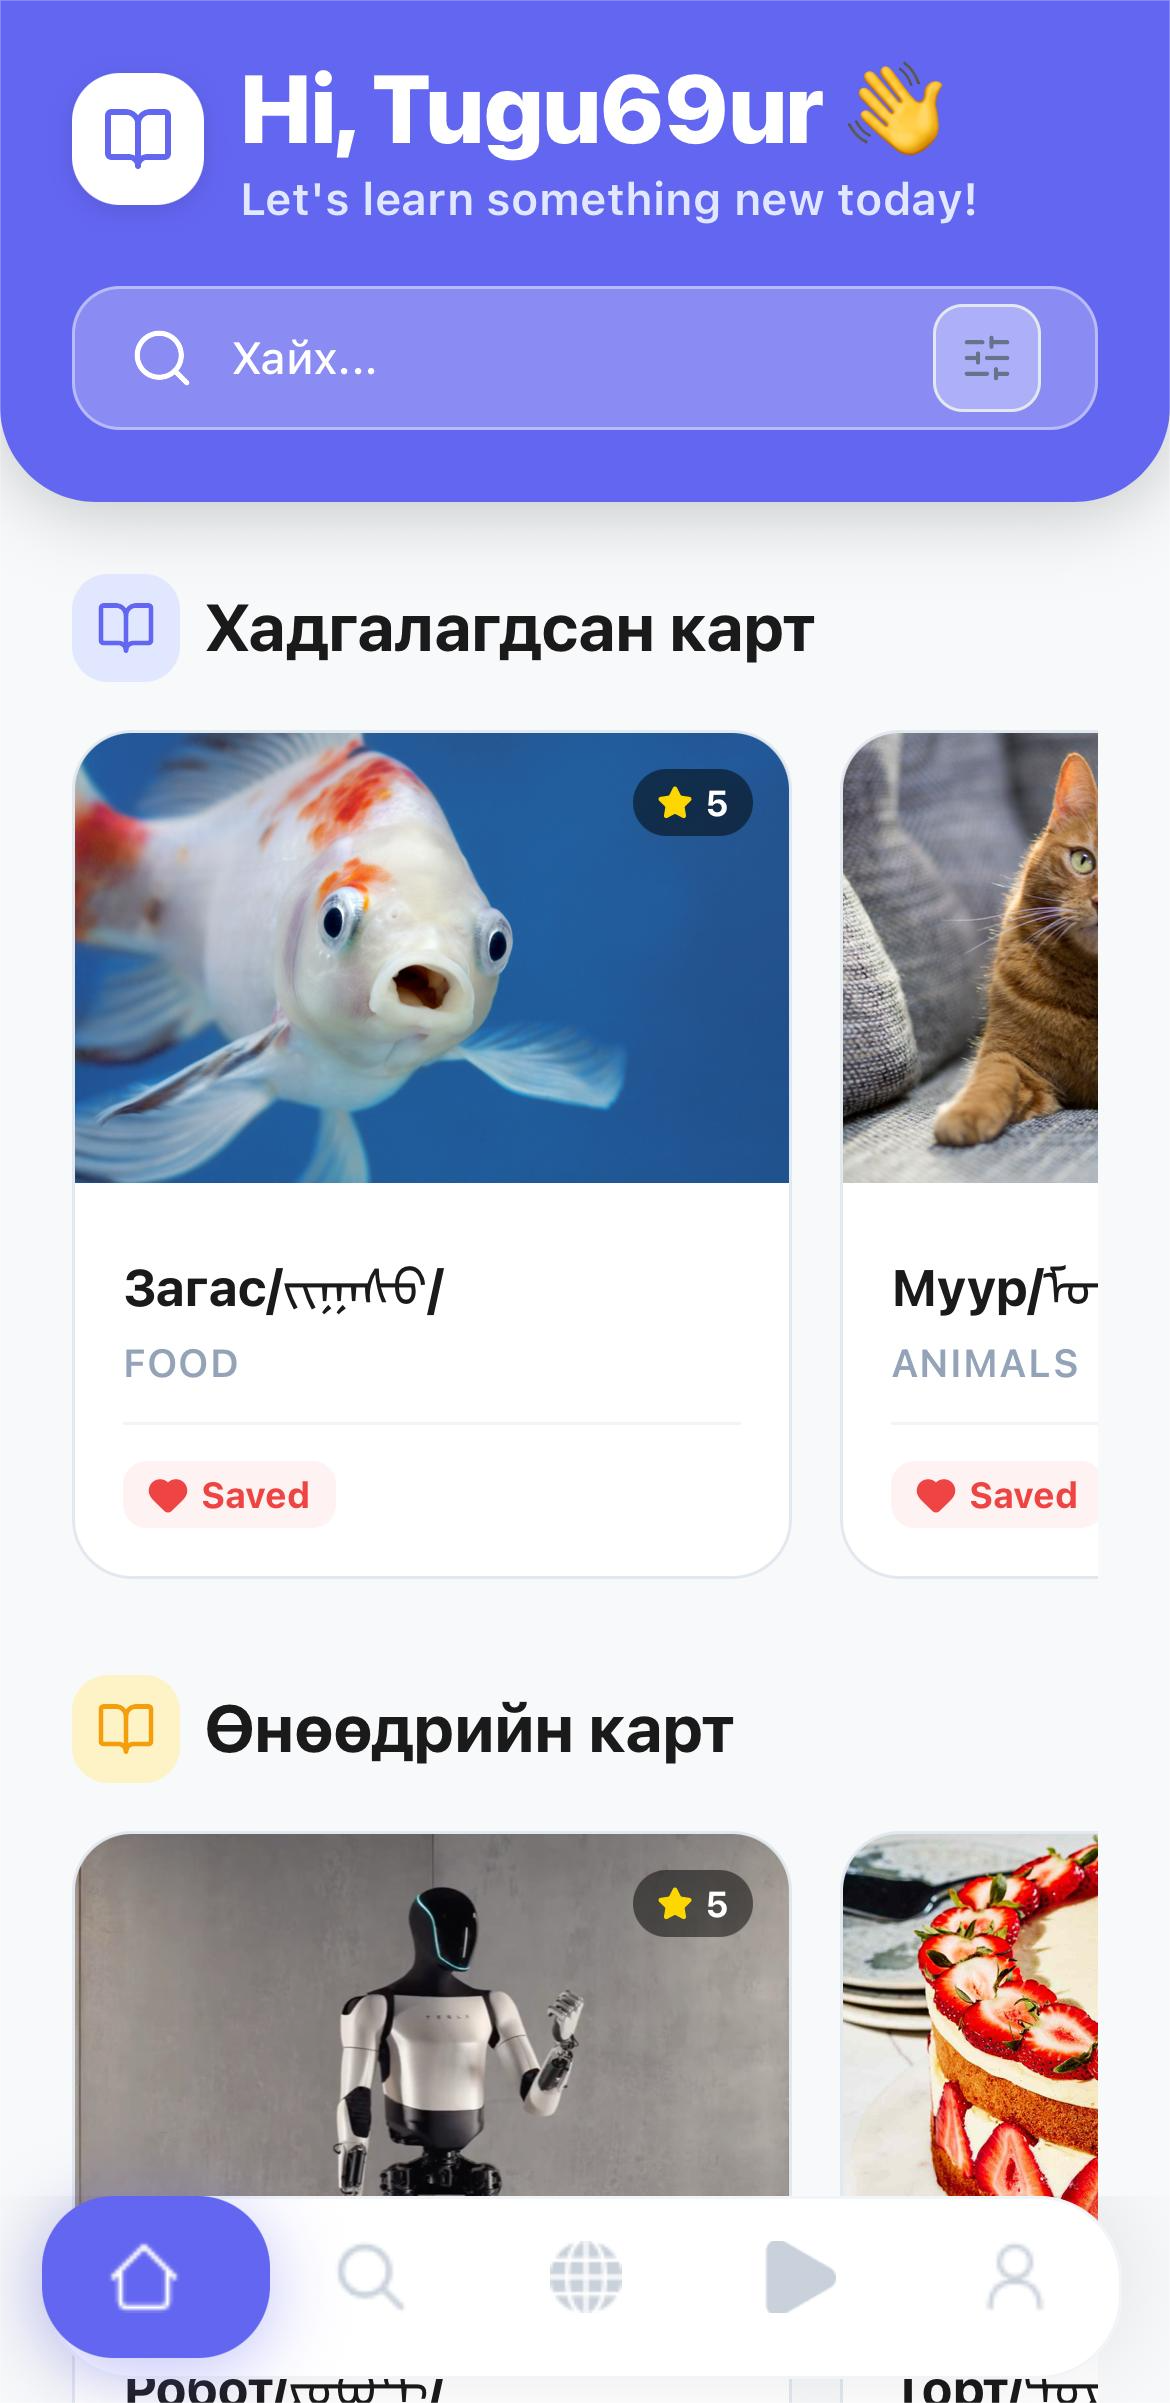
\includegraphics[width=0.35\textwidth]{Figures/pages/home.png}
    \caption{Нүүр дэлгэц – өдрийн үг, streak ба категориор ангилсан картууд.}
    \label{fig:home}
  \end{figure}
}

\newcommand{\figSearchScreen}{%
  \begin{figure}[htbp]
    \centering
    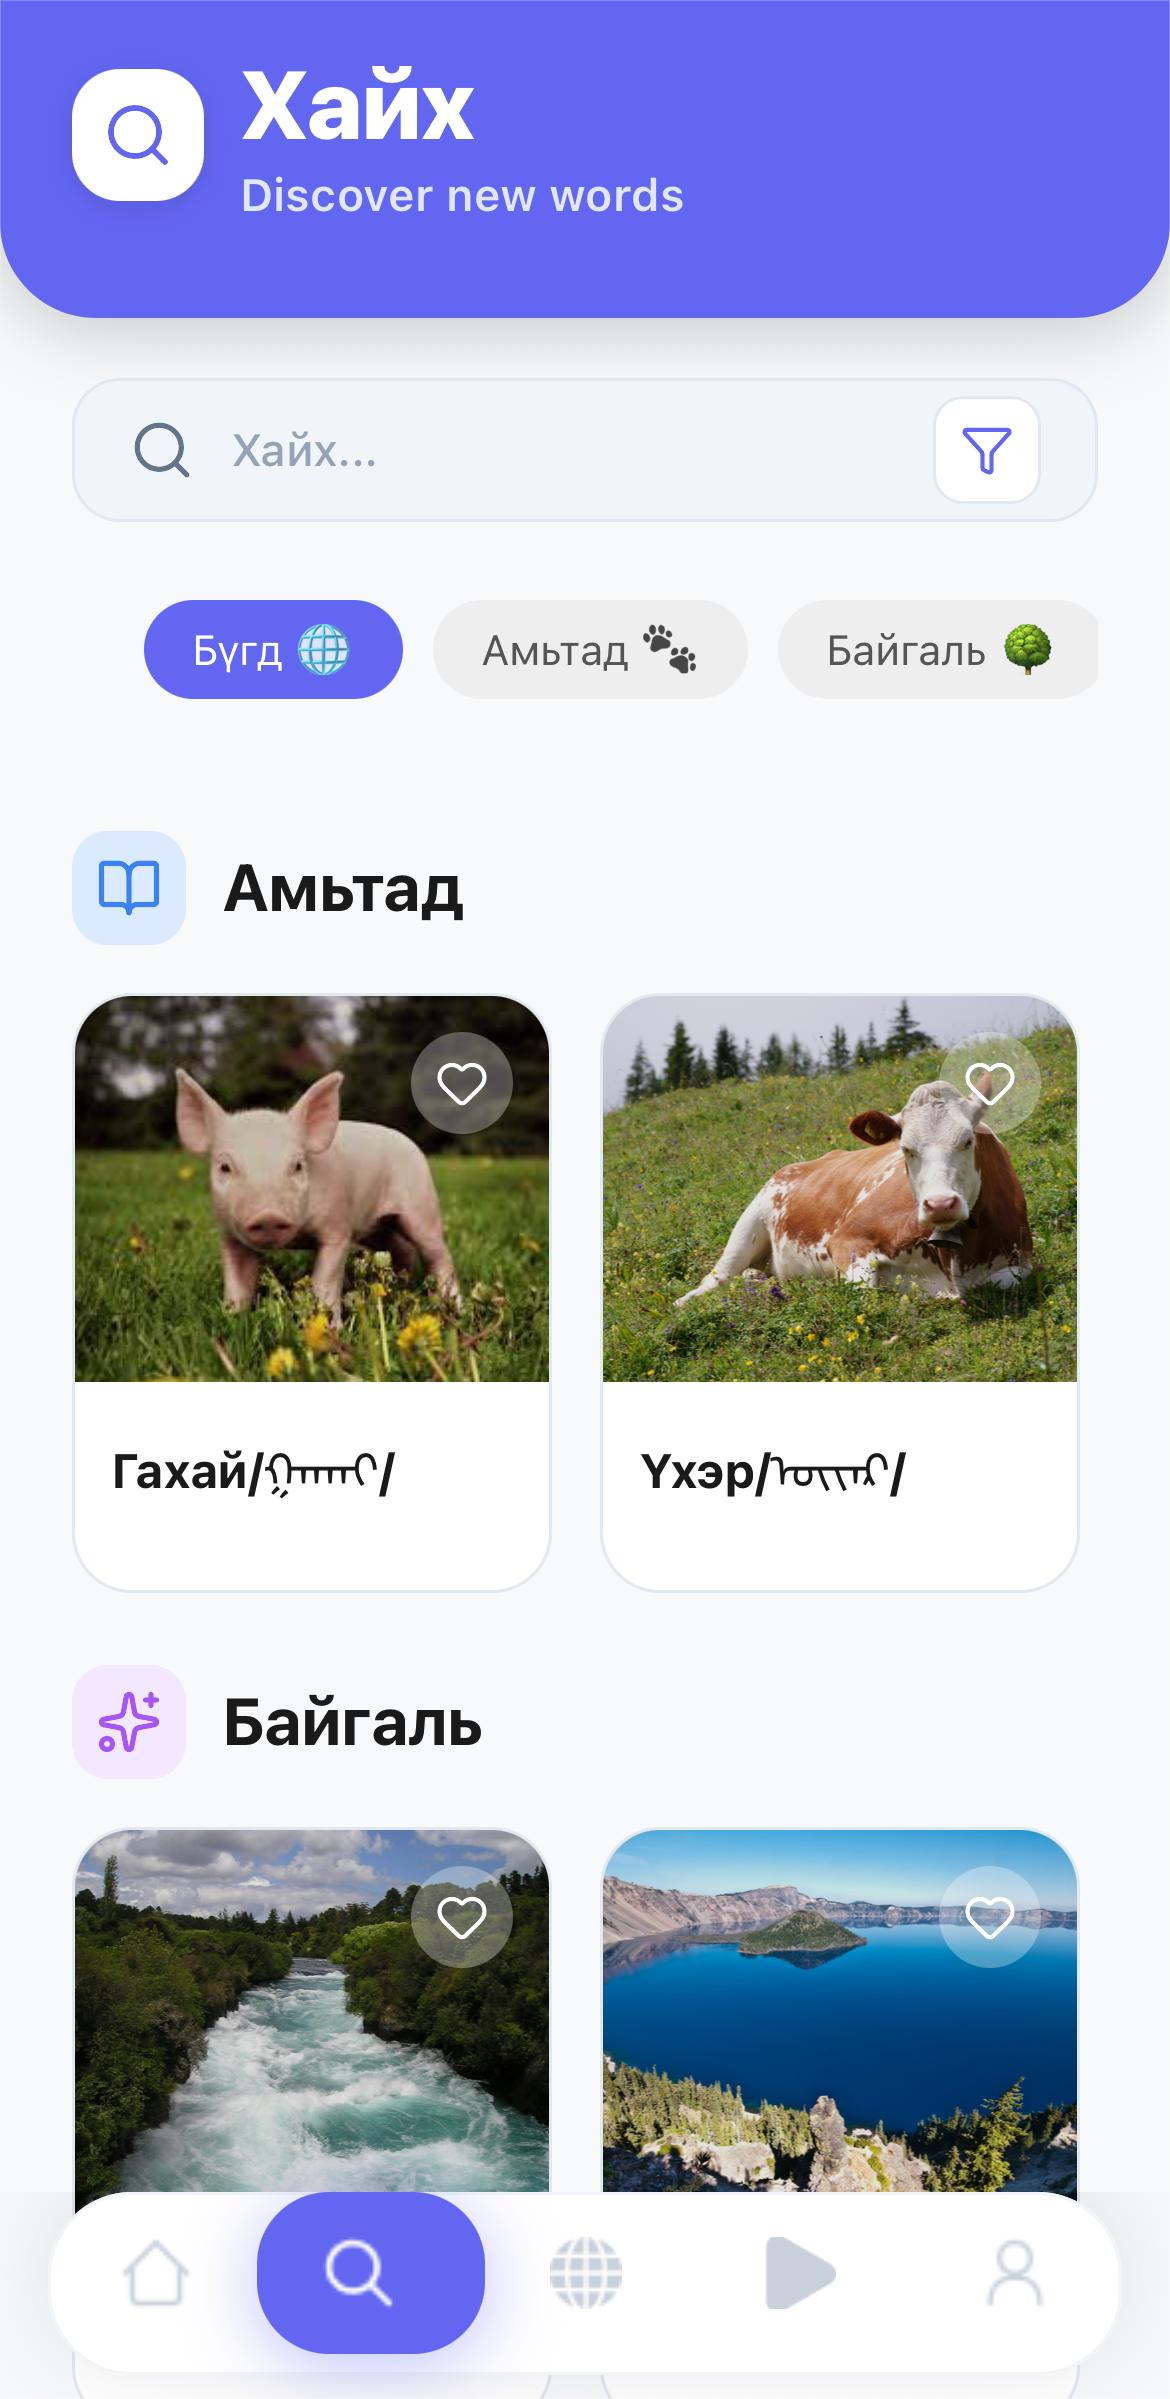
\includegraphics[width=0.35\textwidth]{Figures/pages/search.png}
    \caption{Хайлтын дэлгэц – фонетик, орчуулгаар flashcard хайх интерфейс.}
    \label{fig:search}
  \end{figure}
}

\newcommand{\figProfileScreen}{%
  \begin{figure}[htbp]
    \centering
    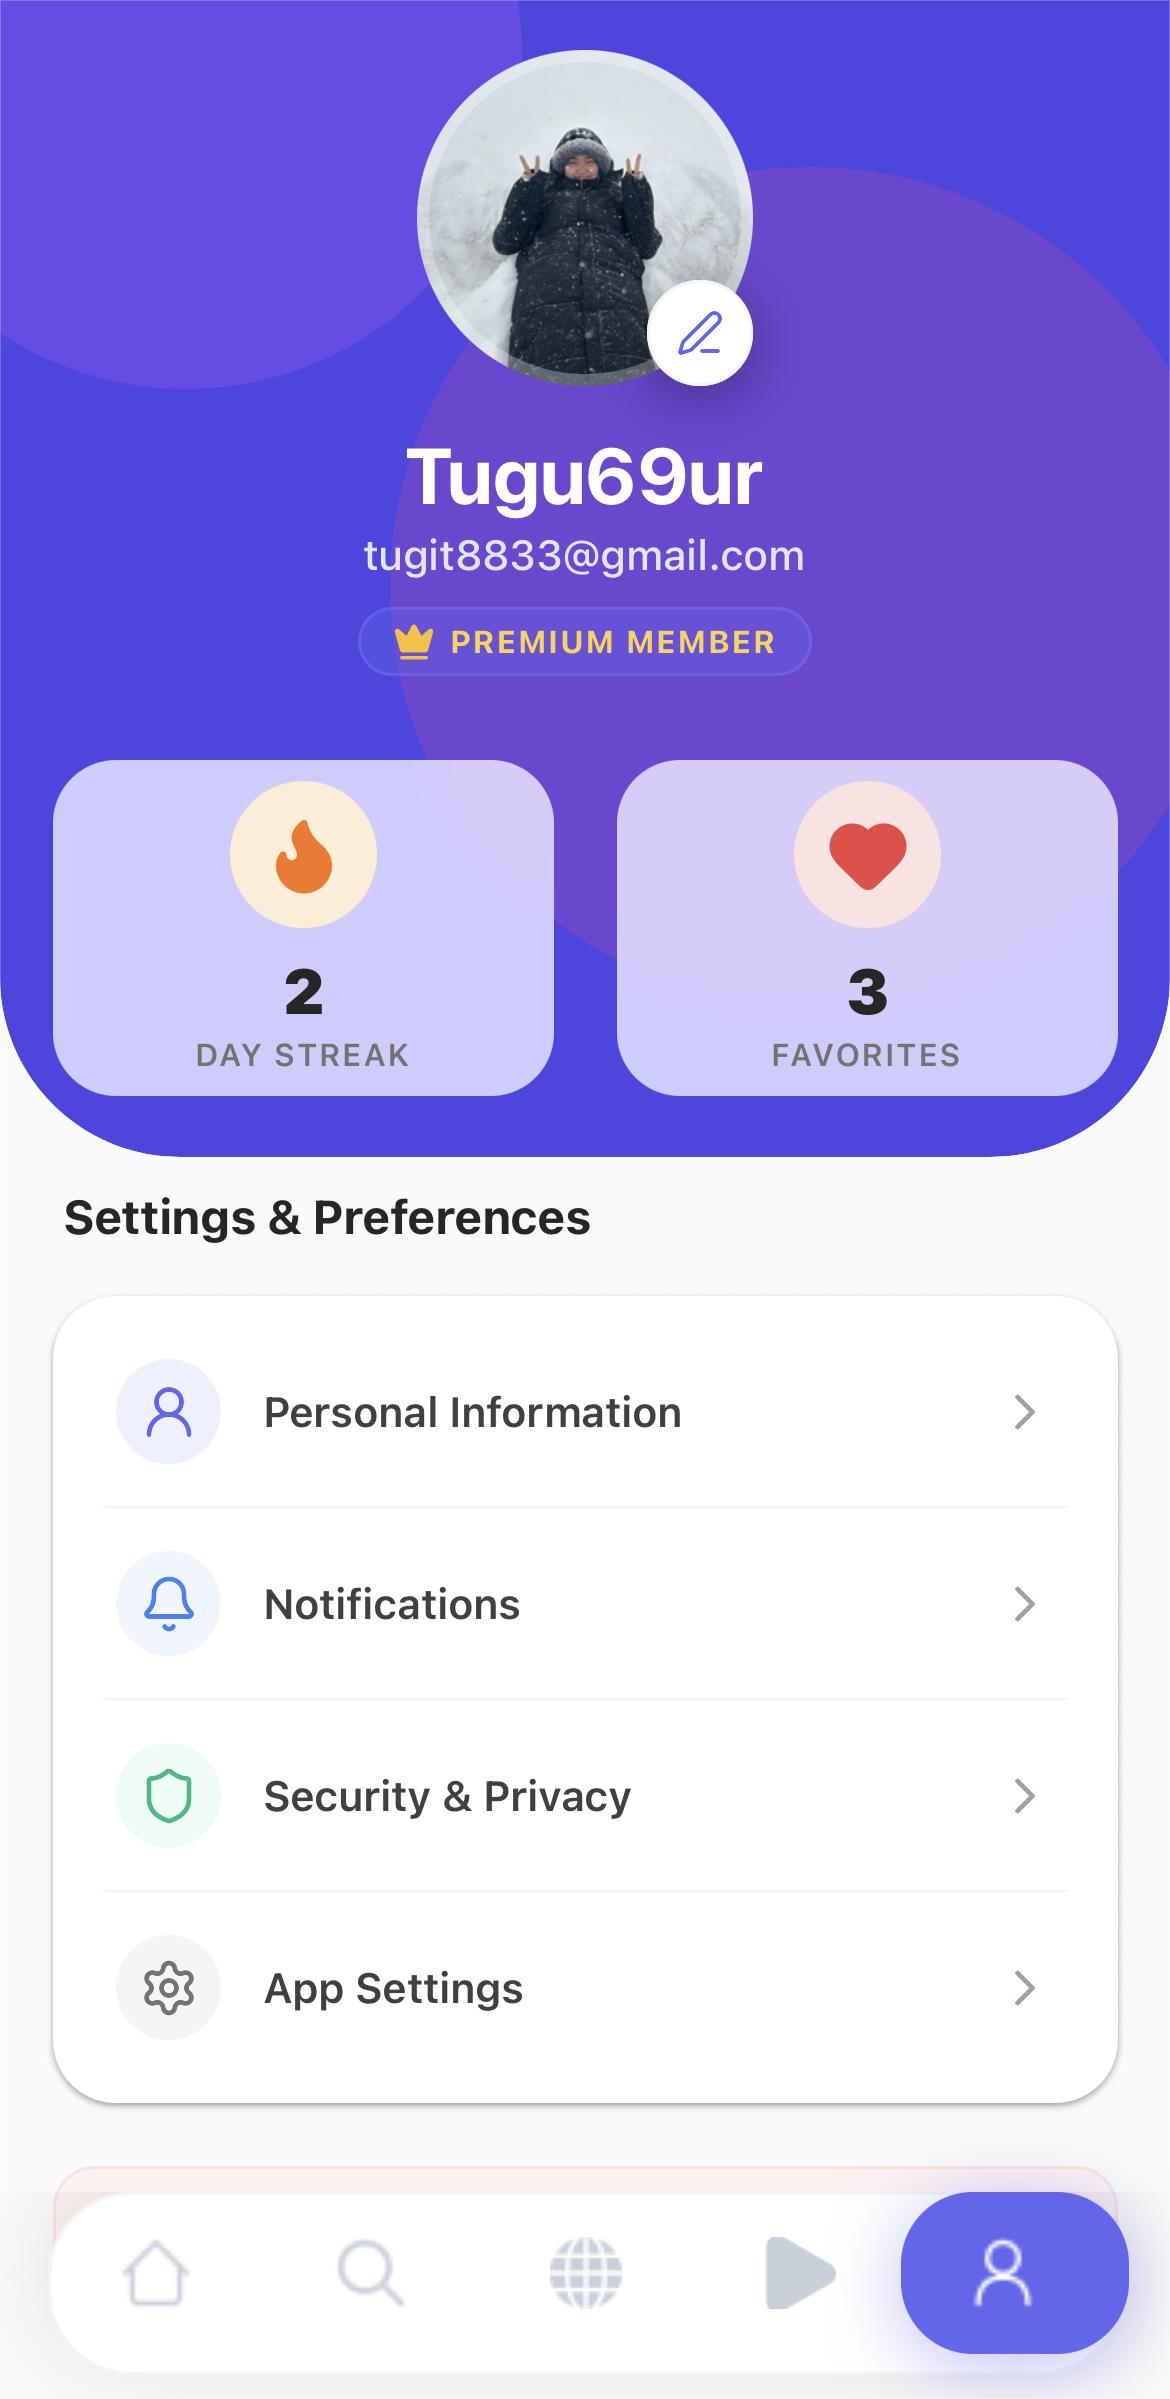
\includegraphics[width=0.35\textwidth]{Figures/pages/profile.png}
    \caption{Профайл дэлгэц – статистик, streak, ахиц дэвшлийн мэдээлэл.}
    \label{fig:profile}
  \end{figure}
}

\newcommand{\figNotificationScreen}{%
  \begin{figure}[htbp]
    \centering
    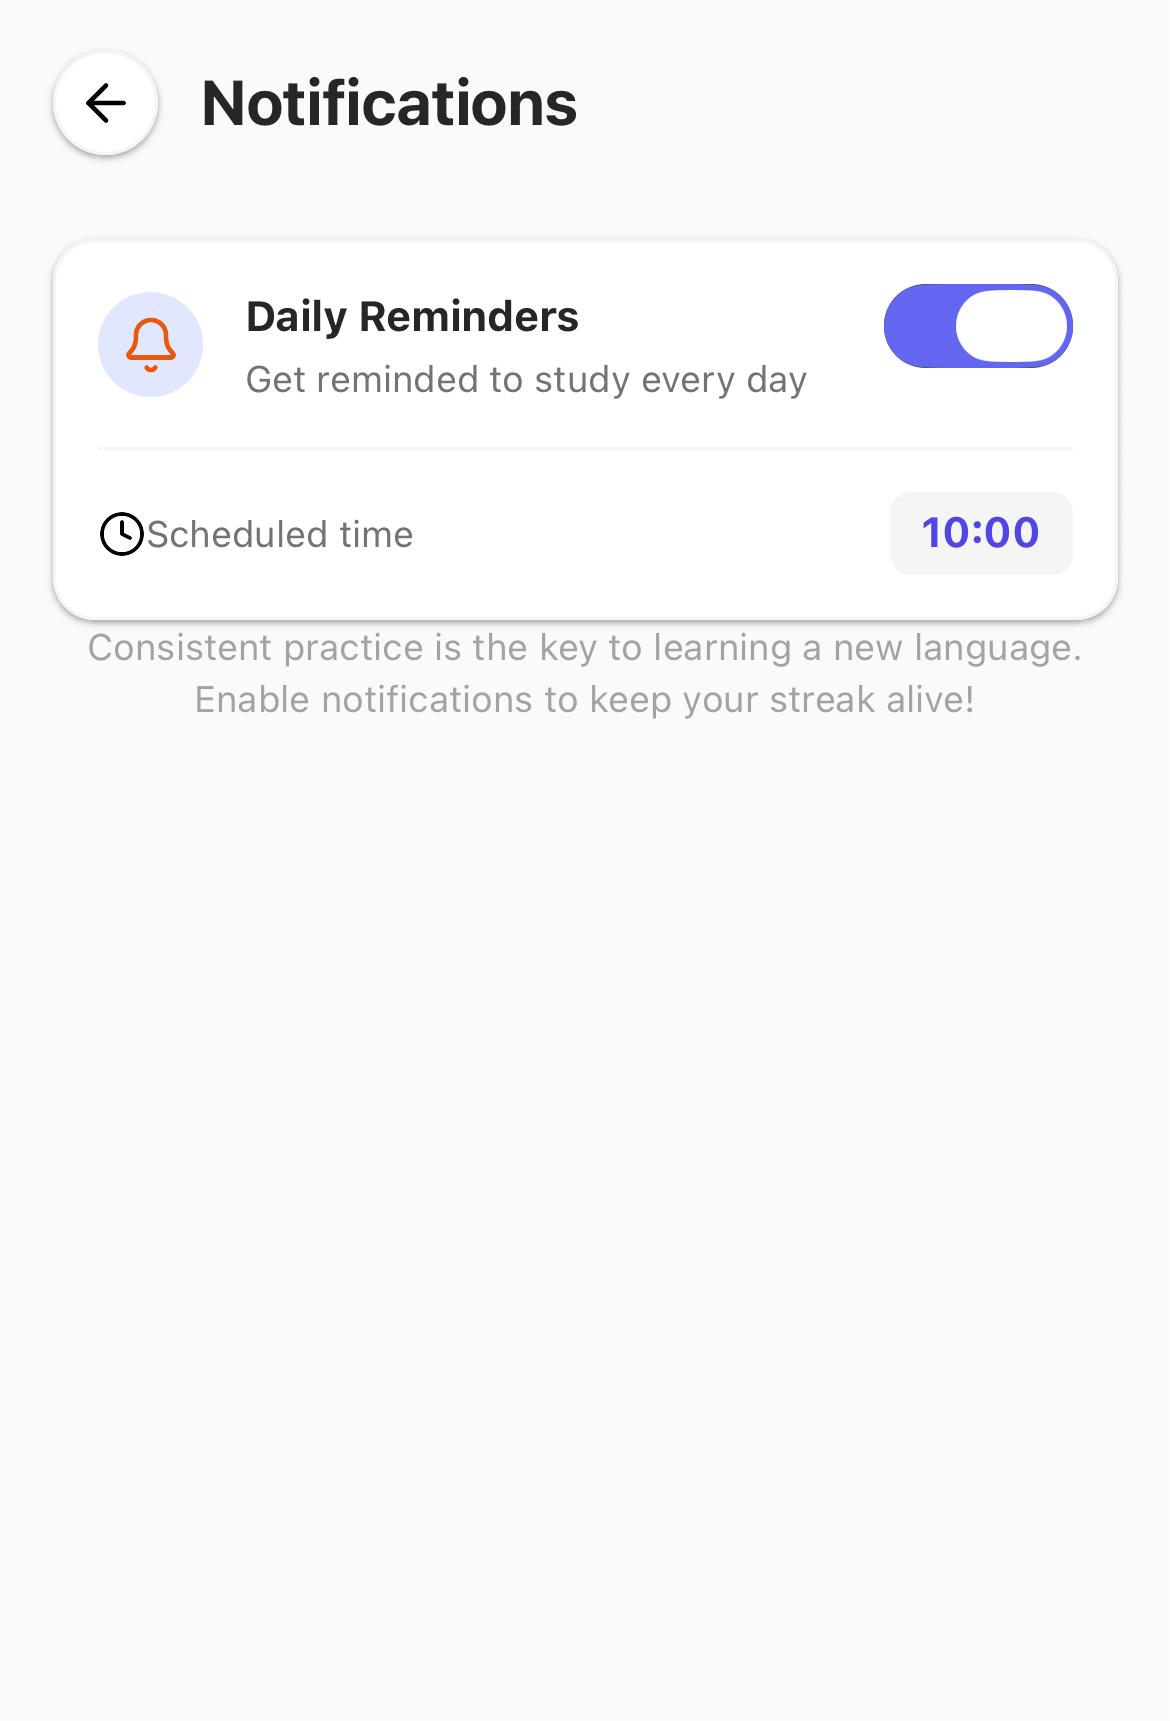
\includegraphics[width=0.35\textwidth]{Figures/pages/notification.png}
    \caption{Мэдэгдлийн дэлгэц – сануулга, streak болон амжилтын мэдэгдлүүд.}
    \label{fig:notifications}
  \end{figure}
}

\newcommand{\figSettingsScreen}{%
  \begin{figure}[htbp]
    \centering
    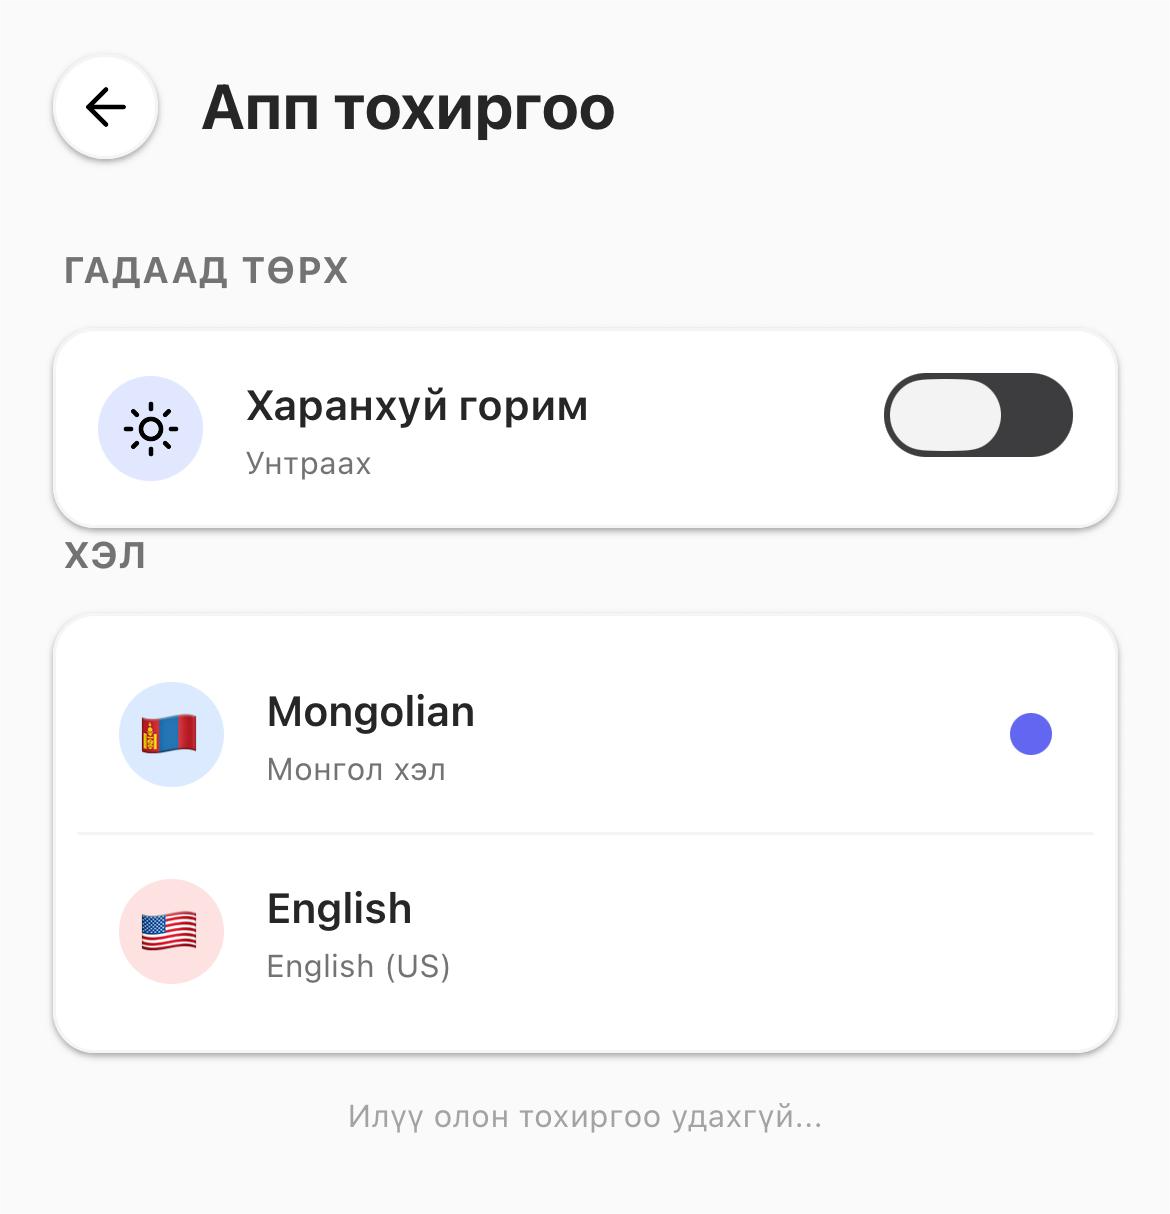
\includegraphics[width=0.35\textwidth]{Figures/pages/settings.png}
    \caption{Тохиргооны дэлгэц – хэл сонголт, theme, мэдэгдэл ба зорилтын тохиргоо.}
    \label{fig:settings}
  \end{figure}
}

\newcommand{\figSecurityPrivacyScreen}{%
  \begin{figure}[htbp]
    \centering
    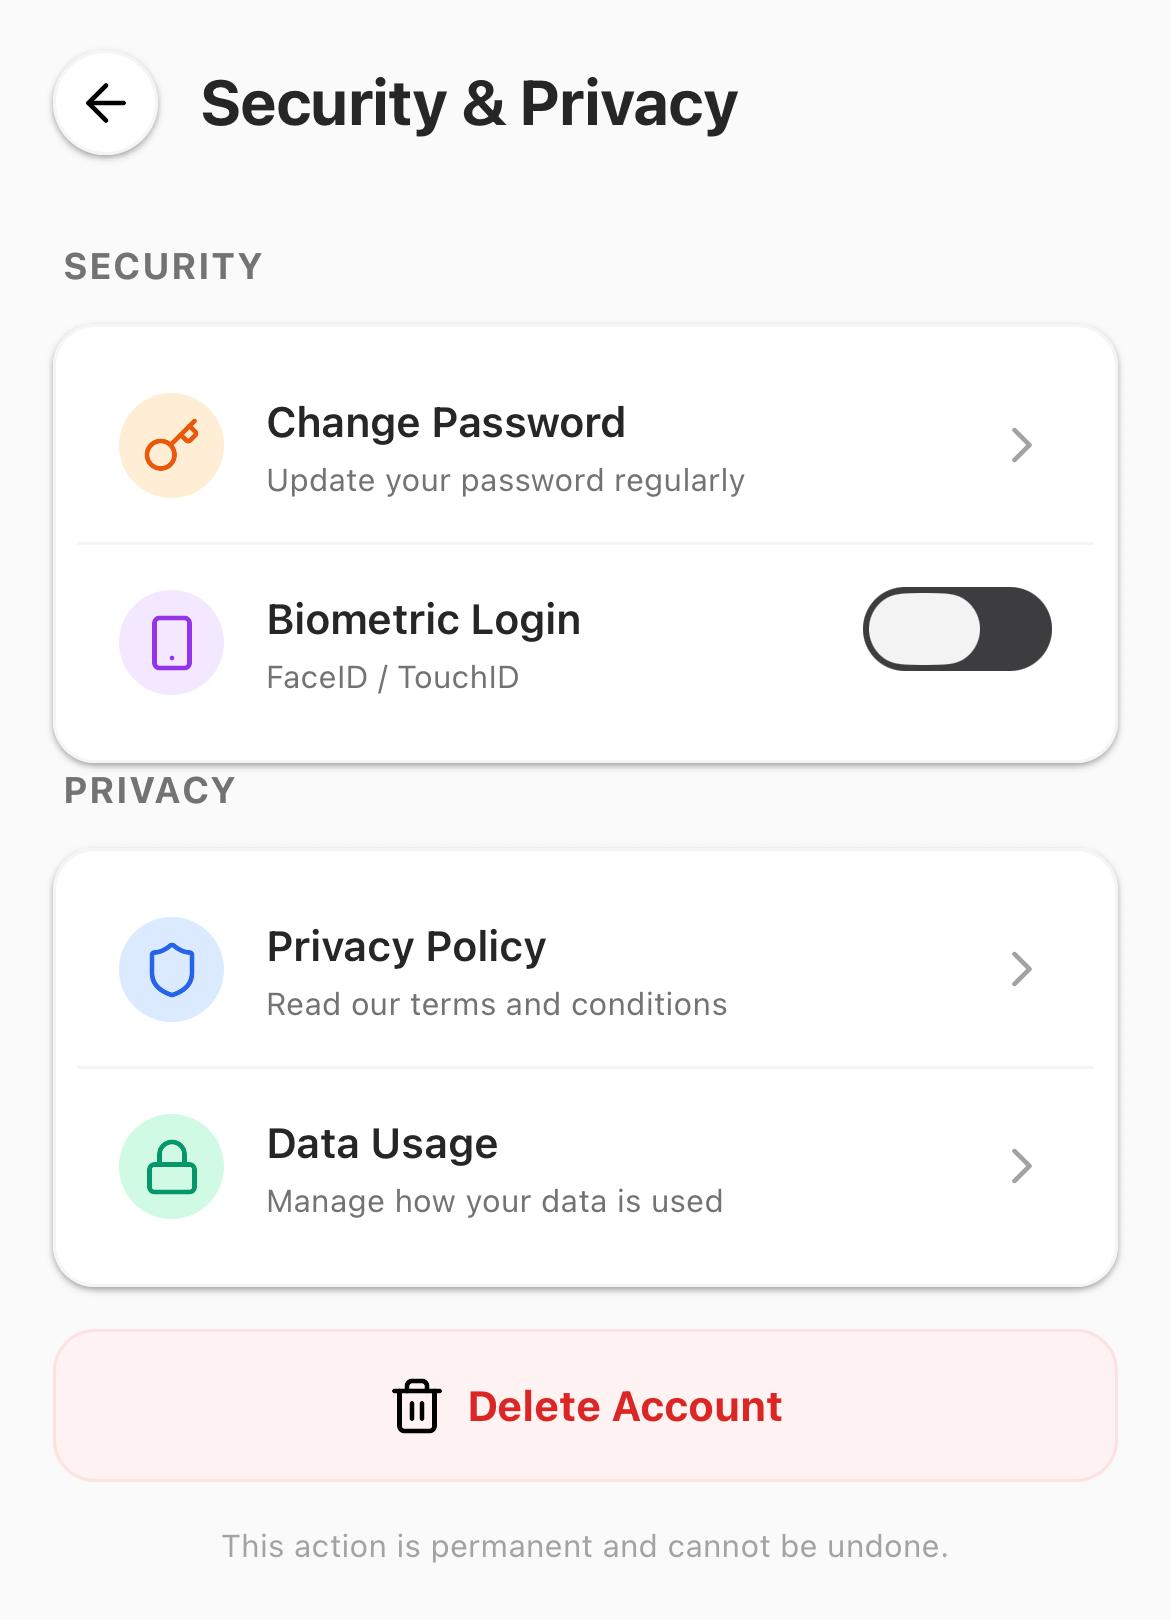
\includegraphics[width=0.35\textwidth]{Figures/pages/security_privacy.png}
    \caption{Аюулгүй байдал ба нууцлалын тохиргооны дэлгэц.}
    \label{fig:security-privacy}
  \end{figure}
}

%==============================================================================
% USER INTERFACE - OCR HANDWRITING RECOGNITION (Chapter 4)
%==============================================================================

\newcommand{\figCameraInputScreen}{%
  \begin{figure}[htbp]
    \centering
    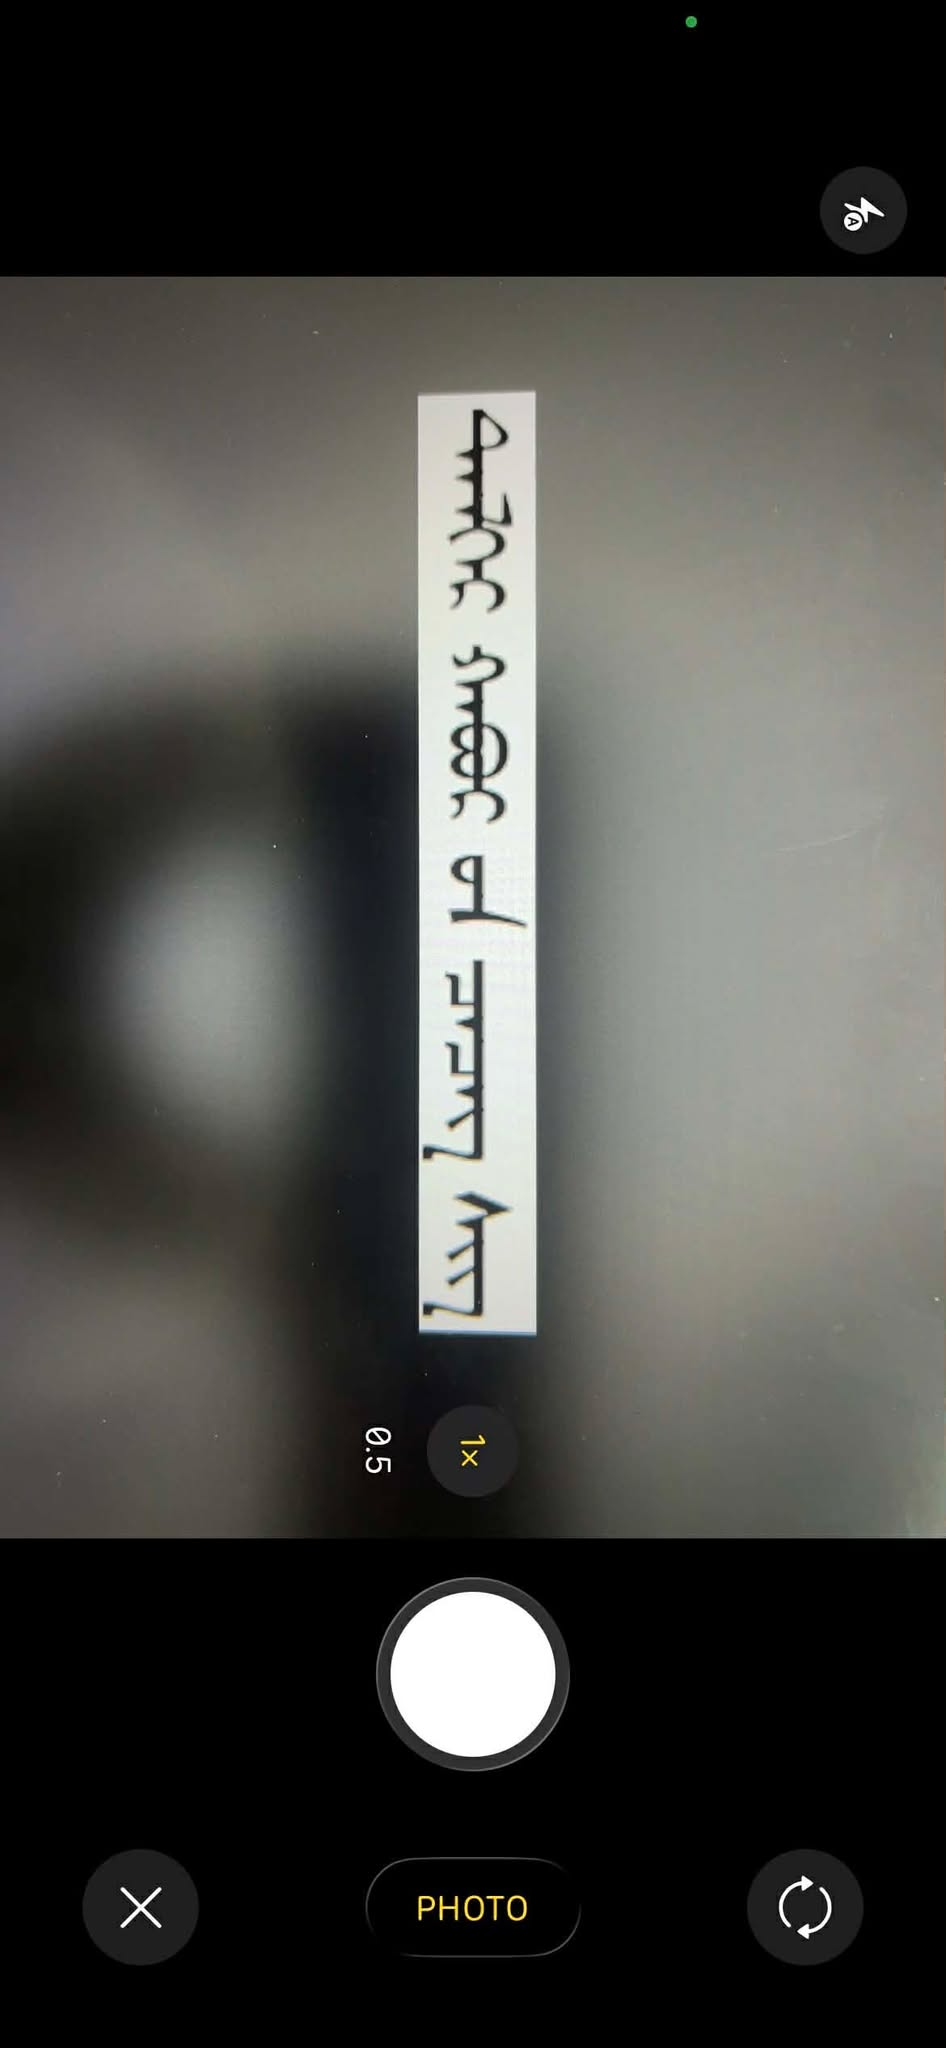
\includegraphics[width=0.35\textwidth]{Figures/pages/camera.jpg}
    \caption{Камераар гар бичвэр оруулах OCR дэлгэц.}
    \label{fig:camera}
  \end{figure}
}

\newcommand{\figHandwritingInput}{%
  \begin{figure}[htbp]
    \centering
    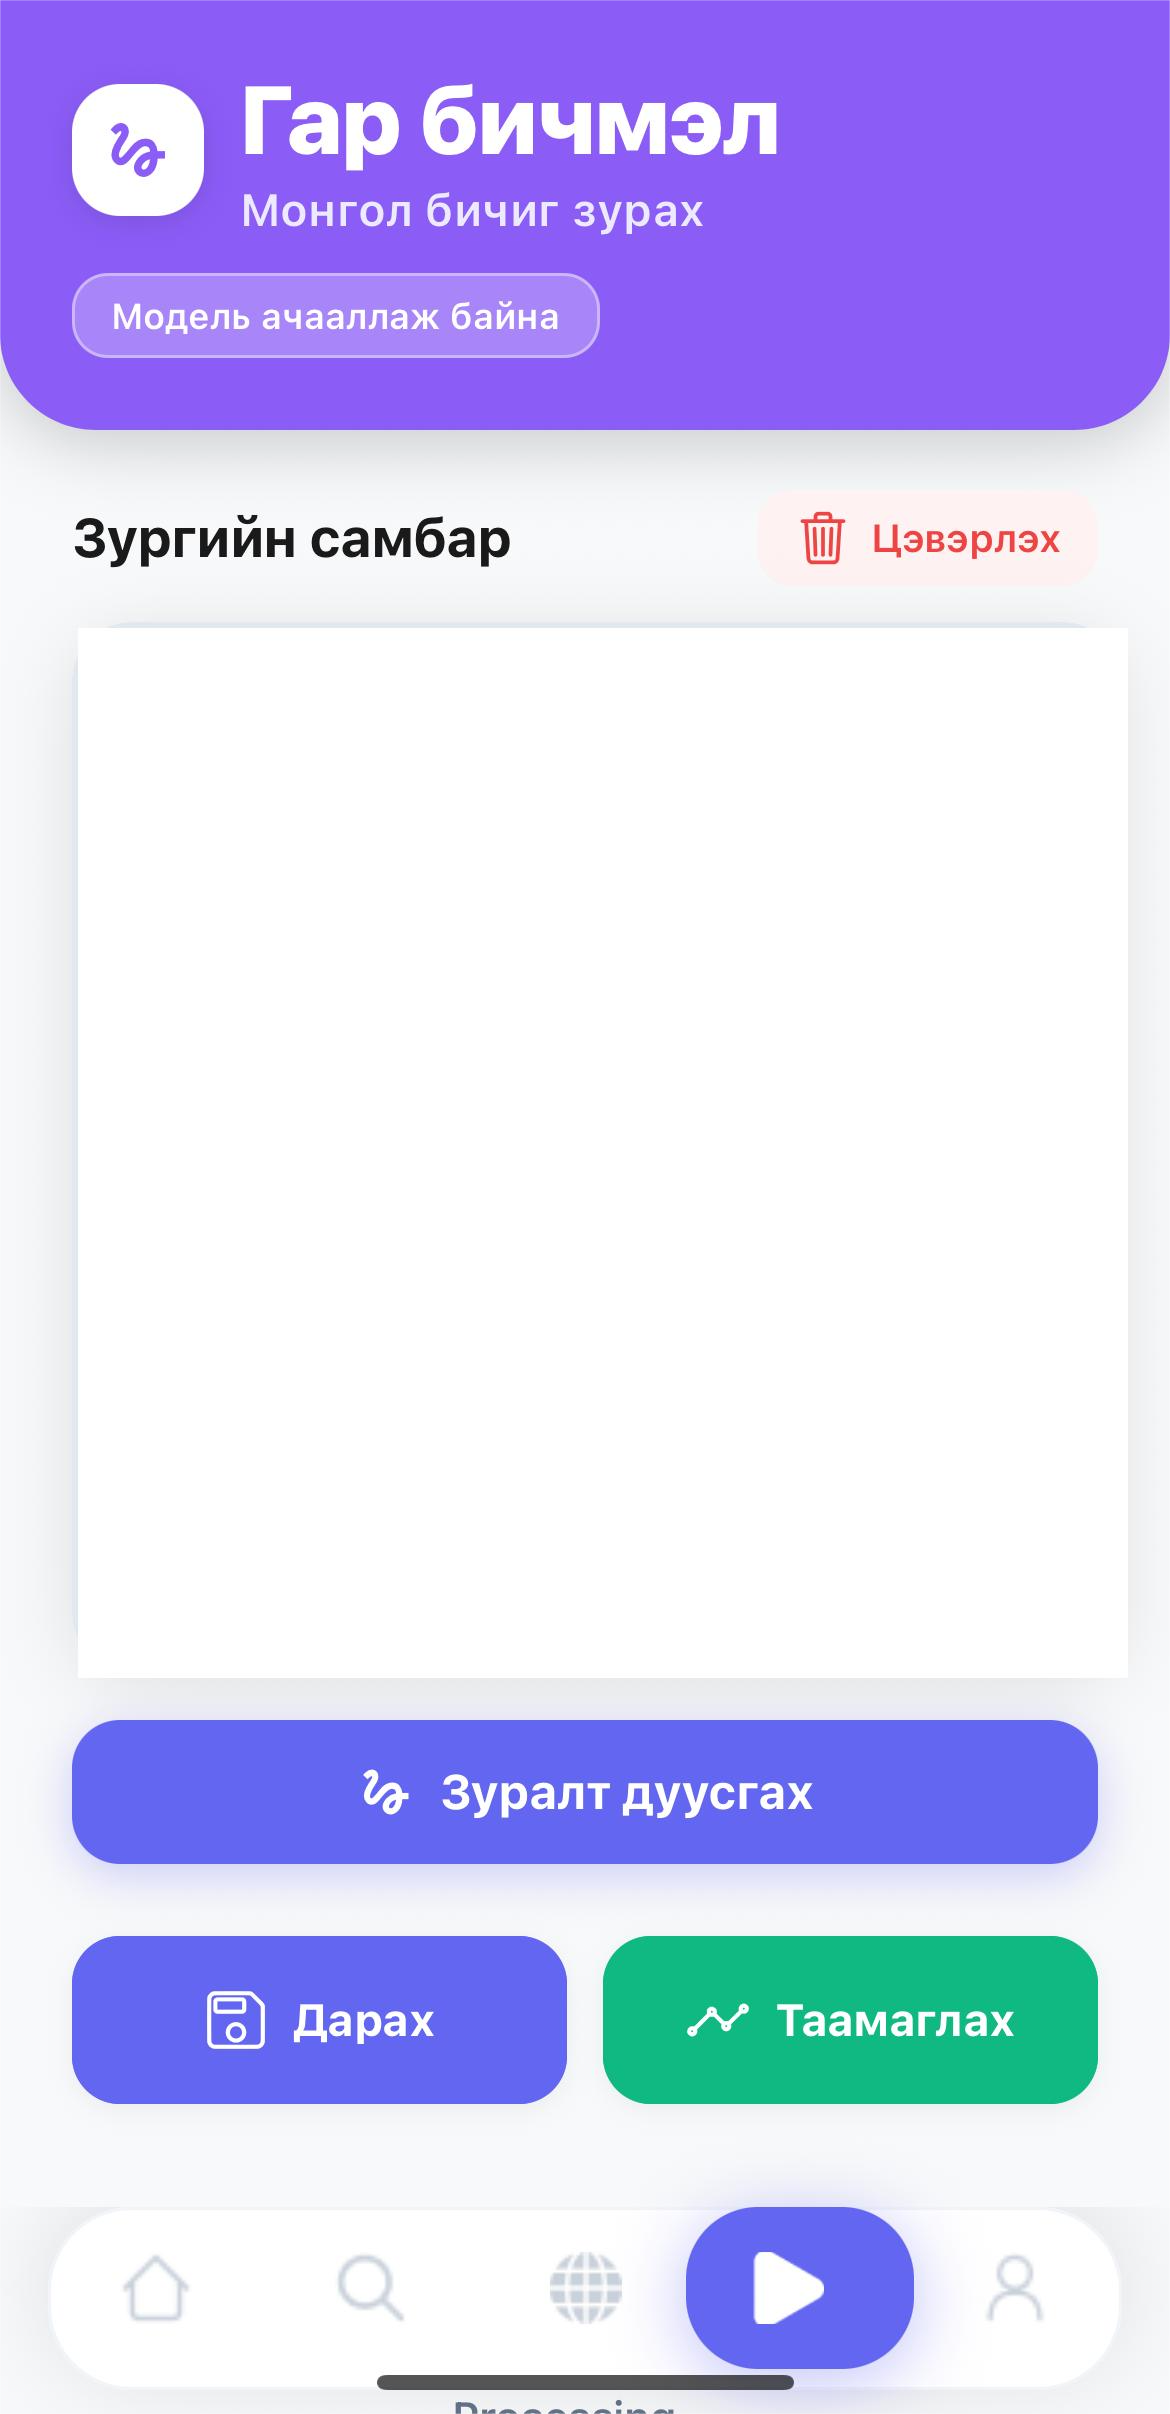
\includegraphics[width=0.35\textwidth]{Figures/pages/handwriting.png}
    \caption{Дэлгэцэн дээр уламжлалт Монгол бичгийг гараар зурах гар бичвэрийн canvas.}
    \label{fig:handwriting}
  \end{figure}
}

\newcommand{\figHandwrittenText}{%
  \begin{figure}[htbp]
    \centering
    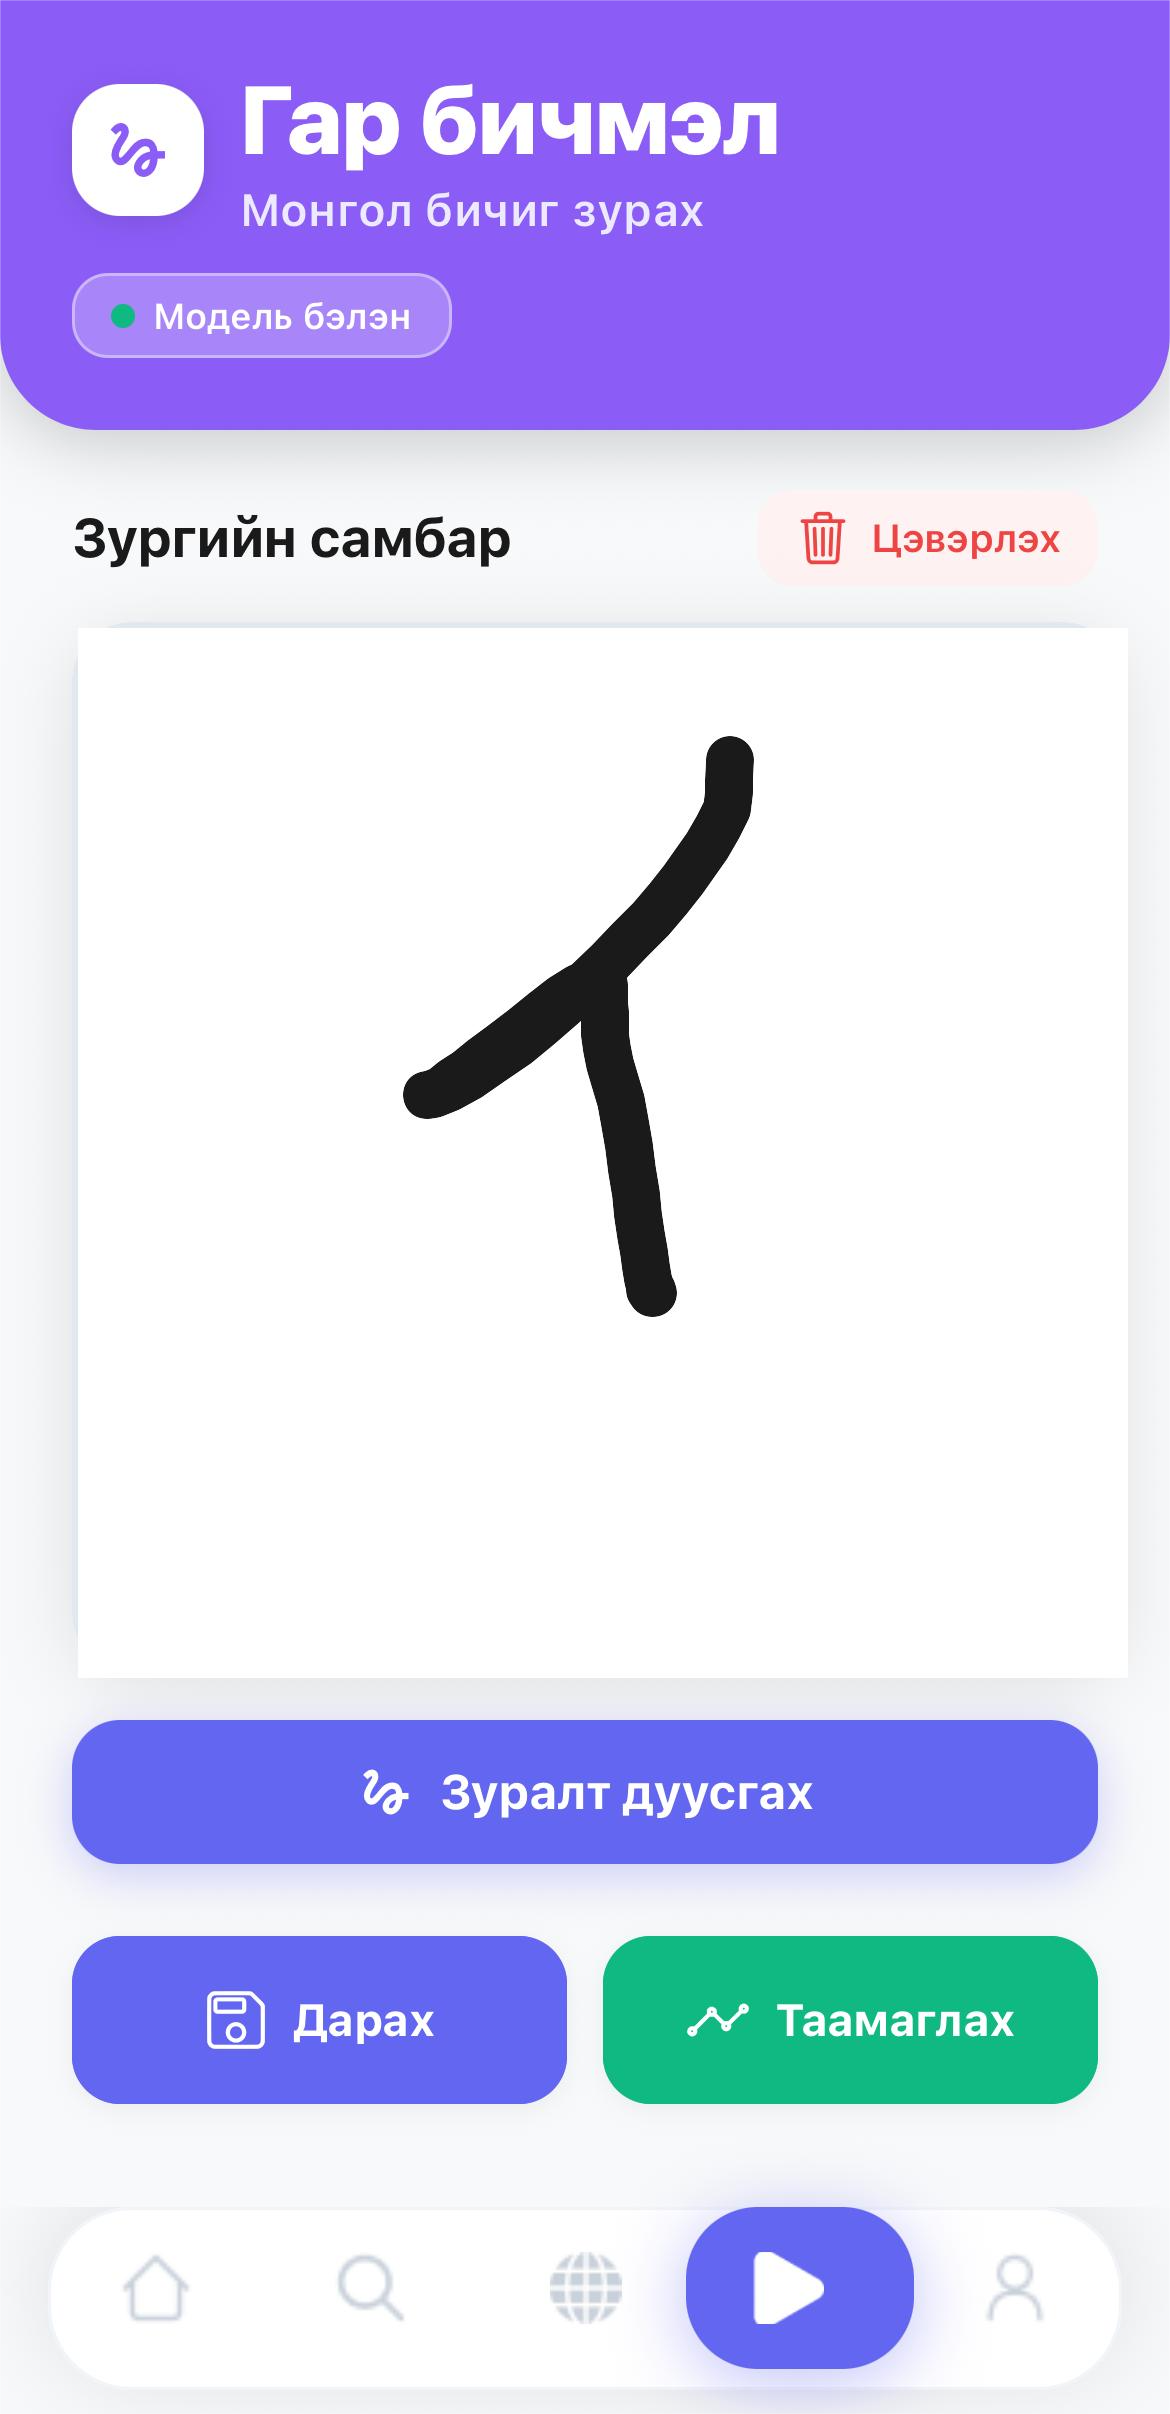
\includegraphics[width=0.35\textwidth]{Figures/pages/handwroten.png}
    \caption{OCR-оор таниулсан гар бичвэрийн үр дүнгийн дэлгэц.}
    \label{fig:handwritten-result}
  \end{figure}
}

\newcommand{\figOCRRegularView}{%
  \begin{figure}[htbp]
    \centering
    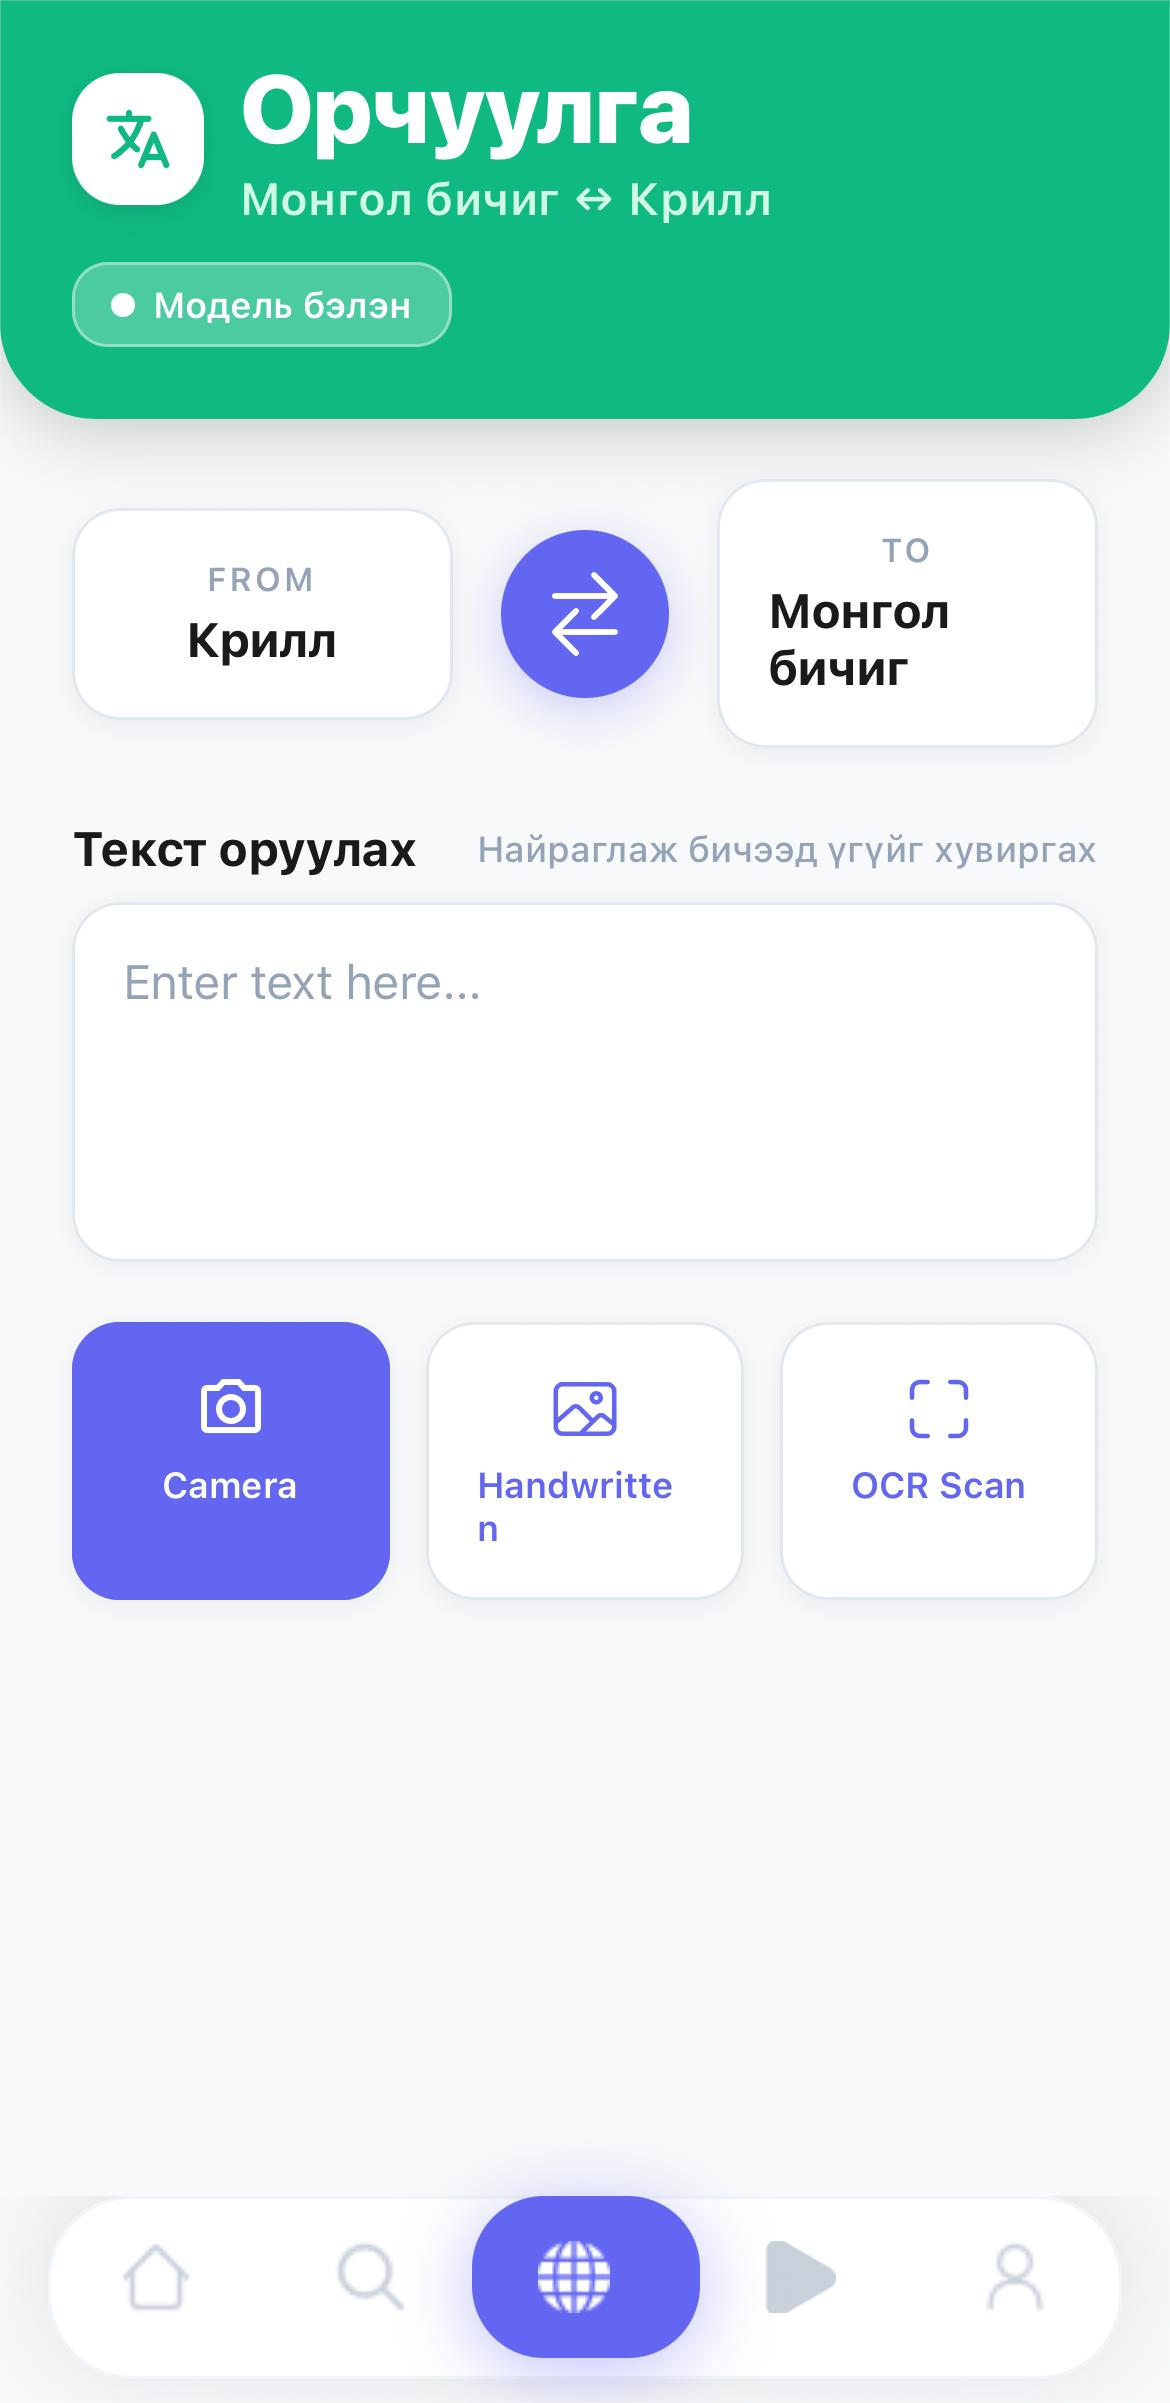
\includegraphics[width=0.35\textwidth]{Figures/pages/ocr_regular_view.png}
    \caption{OCR-оор таниулсан үсгийн дэлгэрэнгүй мэдээлэл бүхий дэлгэц.}
    \label{fig:ocr-regular}
  \end{figure}
}

\newcommand{\figOCRImageToText}{%
  \begin{figure}[htbp]
    \centering
    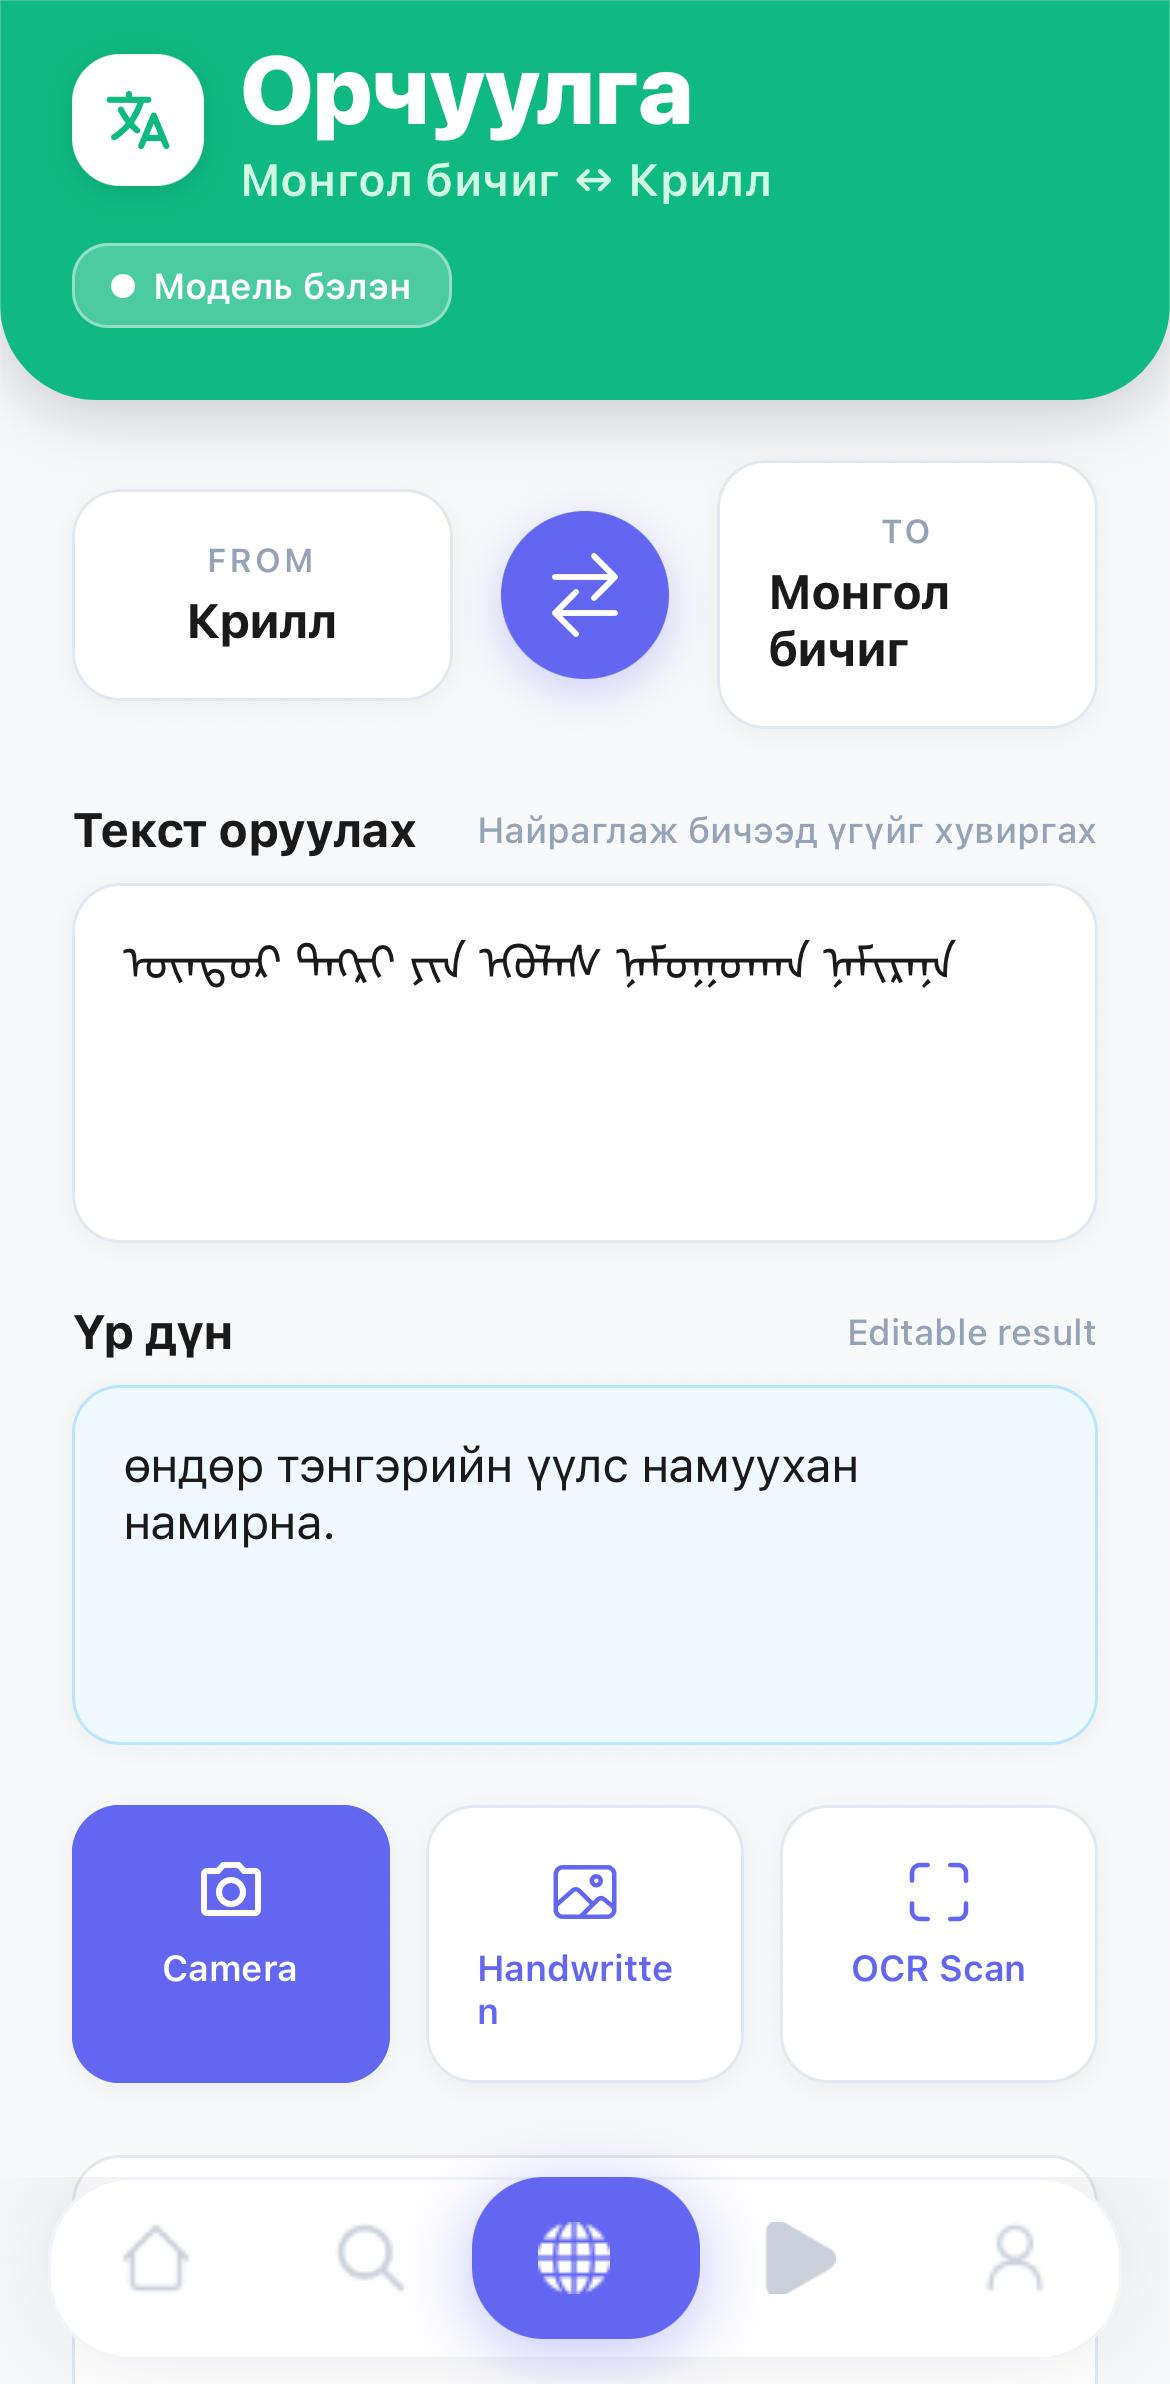
\includegraphics[width=0.35\textwidth]{Figures/pages/ocr_imagetotext.png}
    \caption{Гар бичвэрийг зургаас текст болгон хөрвүүлэх OCR дэлгэц.}
    \label{fig:ocr-image-to-text}
  \end{figure}
}

\newcommand{\figOCRCyrillicScript}{%
  \begin{figure}[htbp]
    \centering
    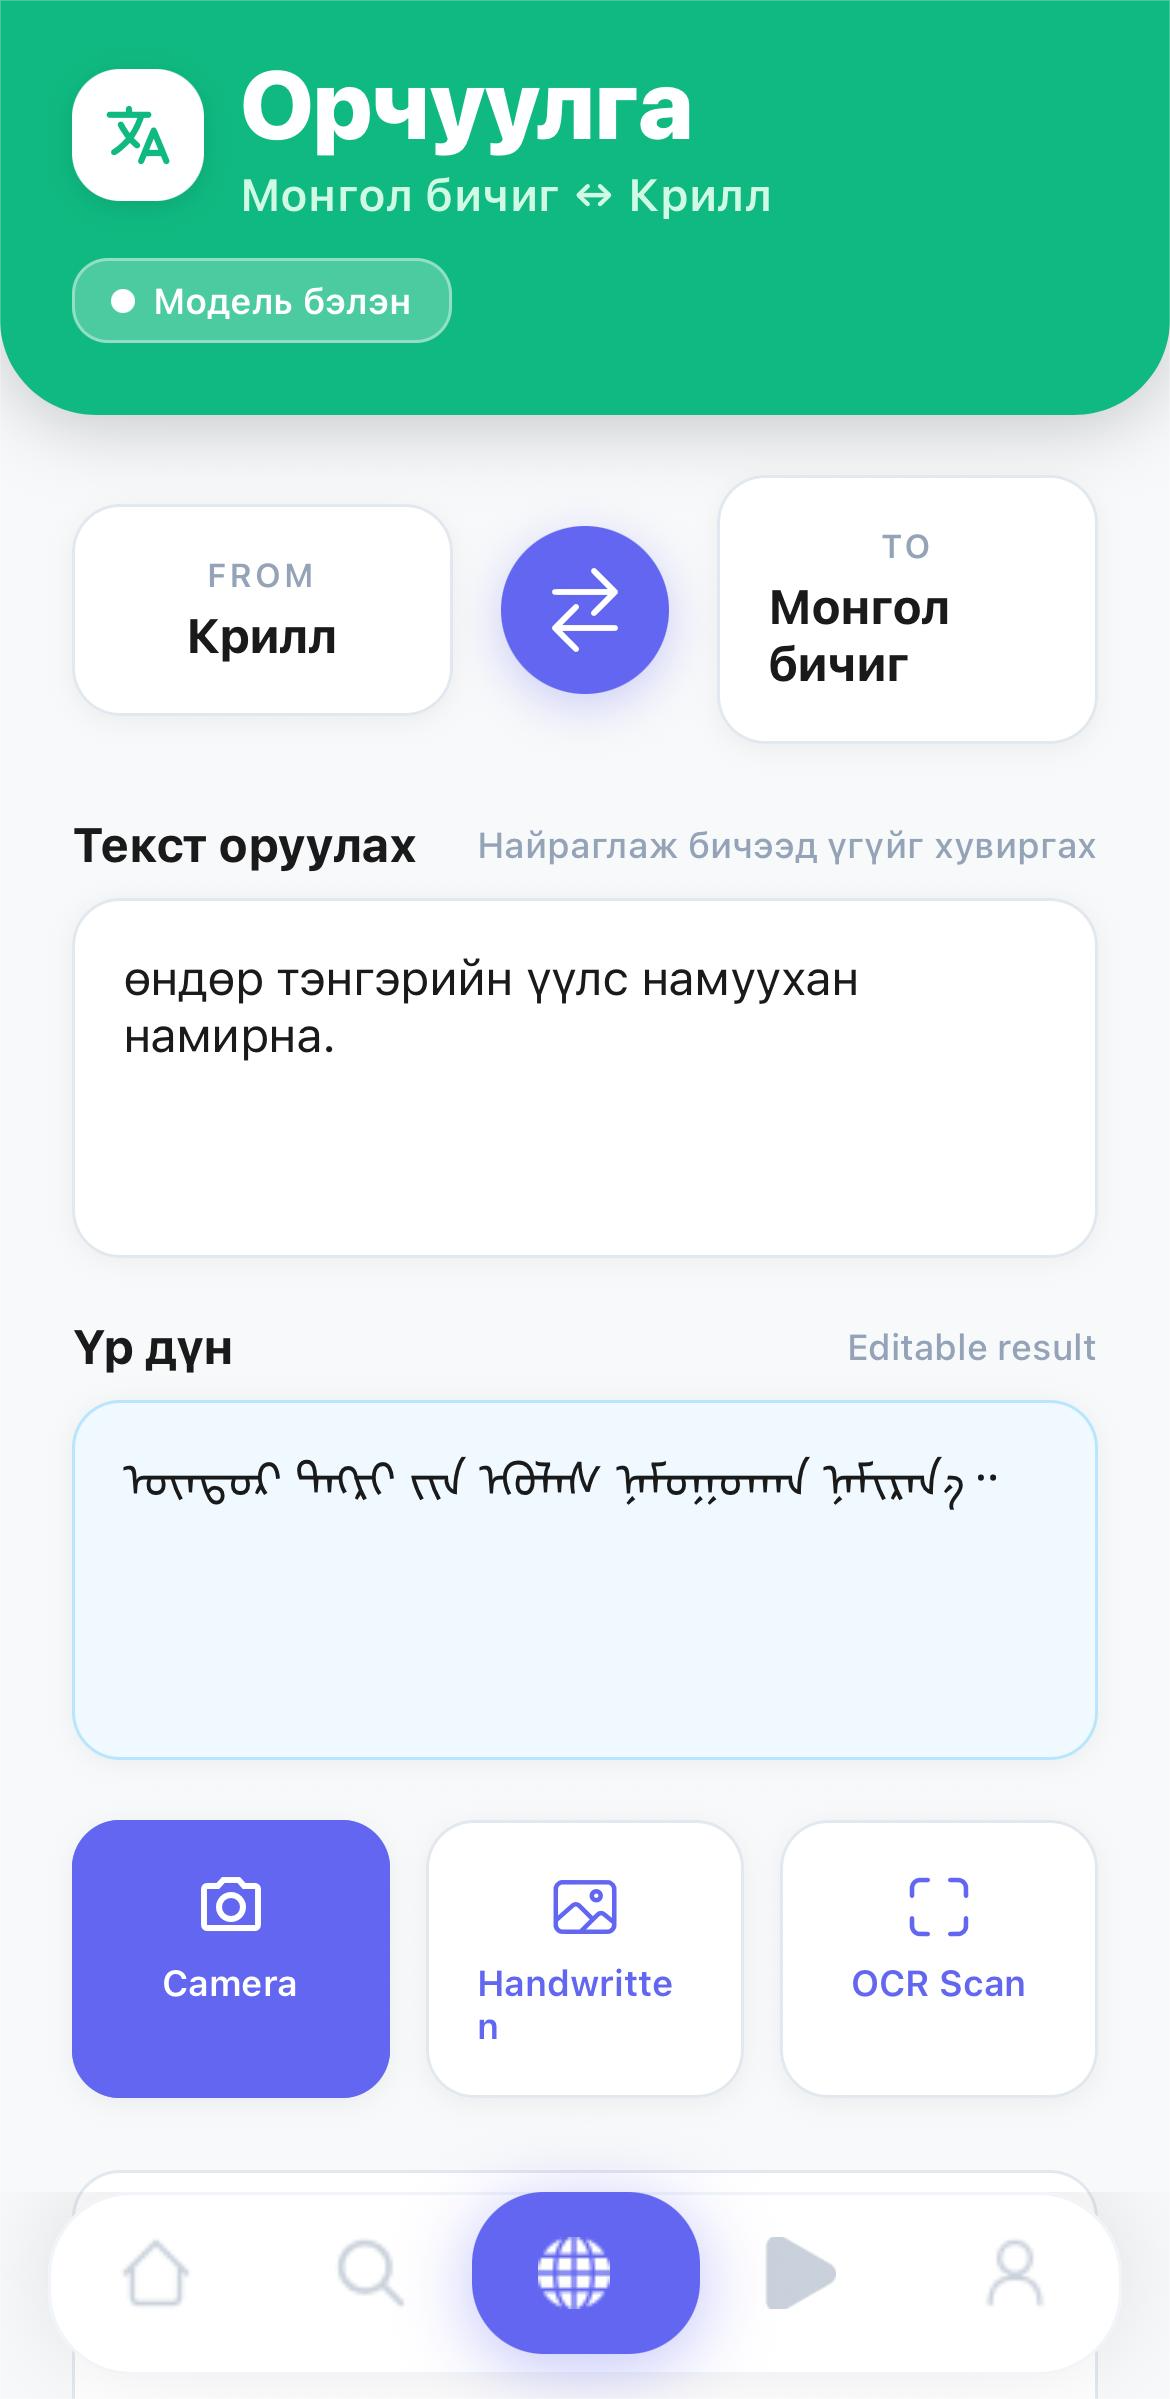
\includegraphics[width=0.35\textwidth]{Figures/pages/ocr_cyrillic_to_script.png}
    \caption{Кирилл бичгээс уламжлалт Монгол бичиг рүү хөрвүүлэх OCR жишээ.}
    \label{fig:ocr-cyrillic}
  \end{figure}
}

%==============================================================================
% MODEL TRAINING AND PERFORMANCE (Chapter 5)
%==============================================================================

\newcommand{\figOCRLearningCurve}{%
  \begin{figure}[H]
    \centering
    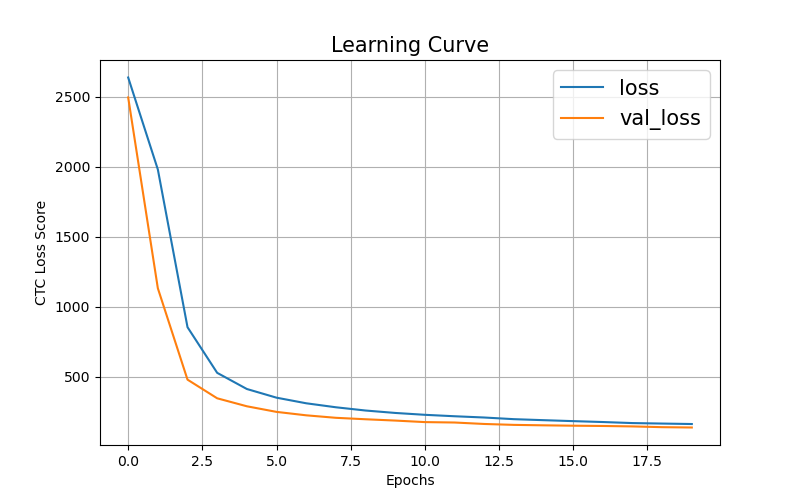
\includegraphics[width=0.85\textwidth]{Figures/whiletrain/OCRModel-LearningCurve.png}
    \caption{TensorFlow.js OCR загварын сургалтын явцын муруйн график (алдагдал болон үнэн зөвийн хувь).}
    \label{fig:learning-curve}
  \end{figure}
}

\newcommand{\figTrainingEpochs}{%
  \begin{figure}[H]
    \centering
    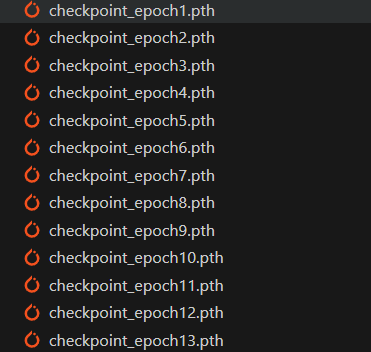
\includegraphics[width=0.85\textwidth]{Figures/whiletrain/epochs.png}
    \caption{OCR загварын сургалтын epoch бүрийн алдагдал, үнэн зөвийн өөрчлөлтийн график.}
    \label{fig:epochs}
  \end{figure}
}

\newcommand{\figModelSegmentation}{%
  \begin{figure}[H]
    \centering
    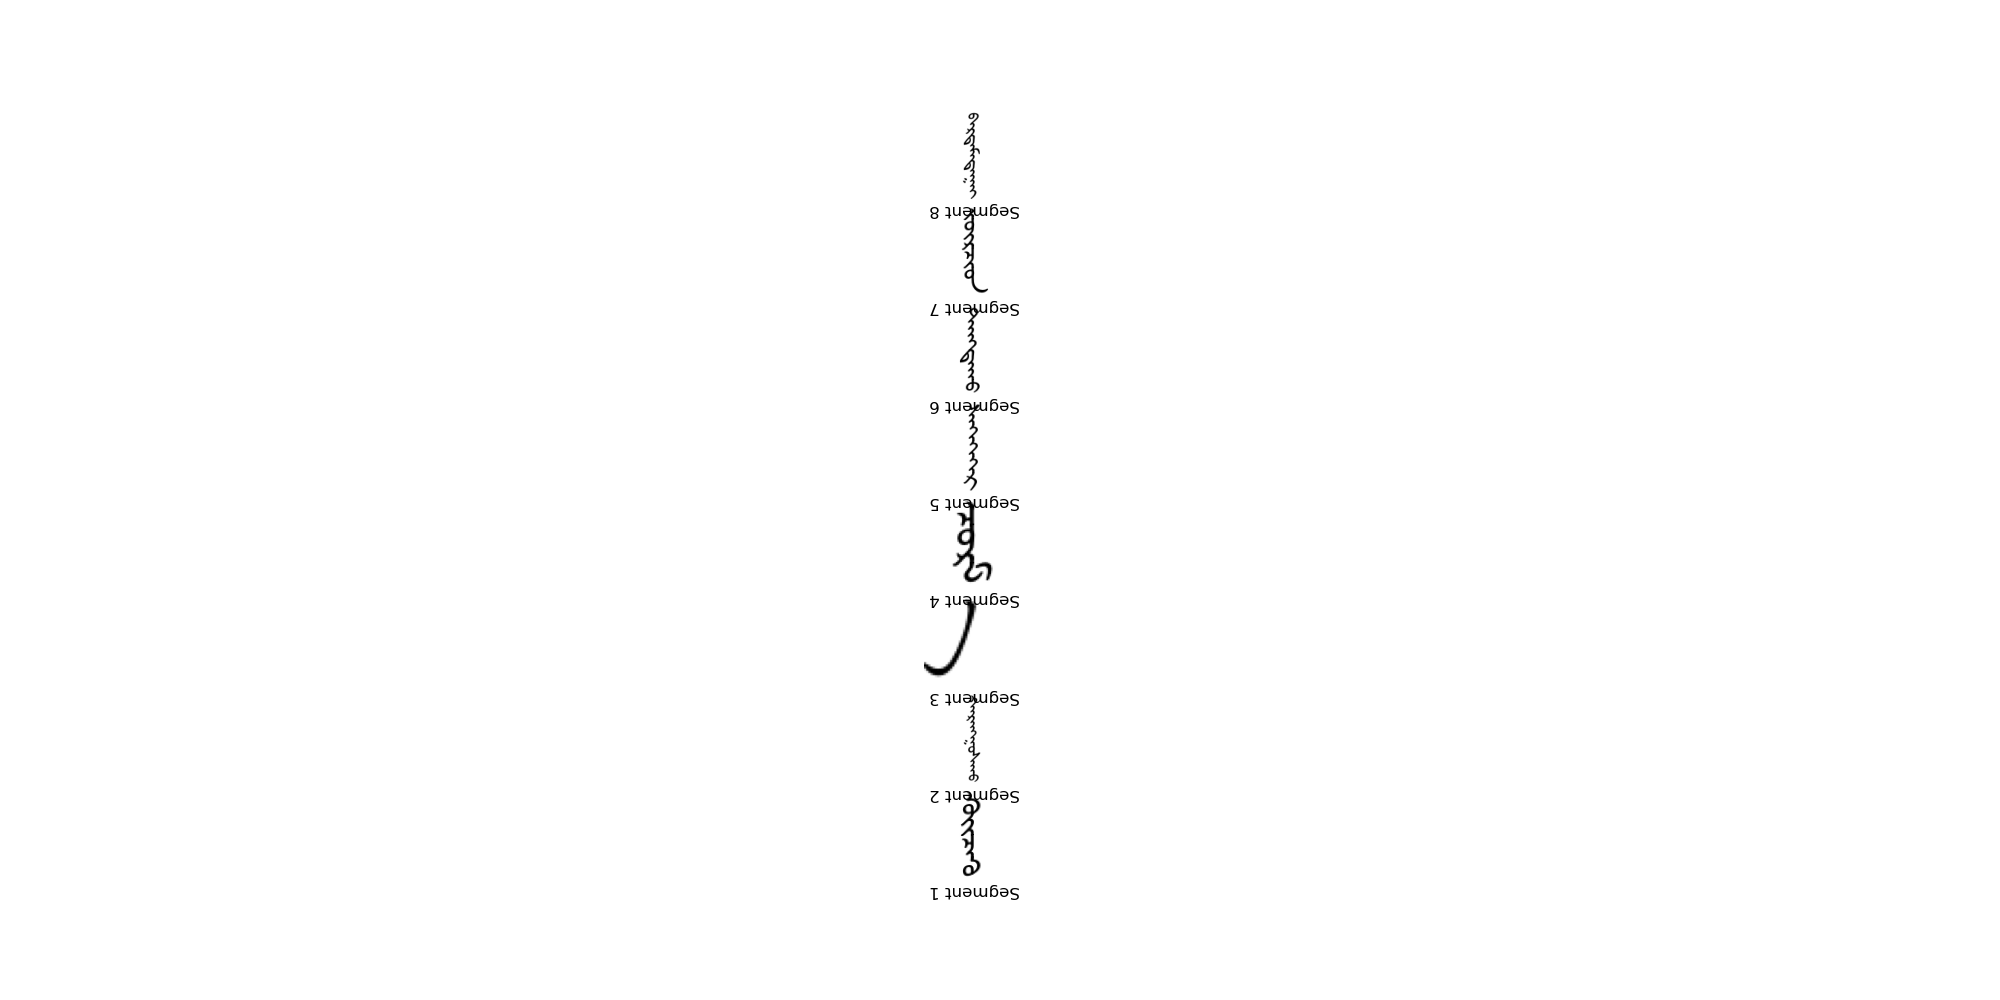
\includegraphics[width=0.85\textwidth]{Figures/whiletrain/all_segments.png}
    \caption{OCR загварын тэмдэгт тусгаарлах (segmentation) жишээ зургийн цуглуулга.}
    \label{fig:segmentation}
  \end{figure}
}

\newcommand{\figLineInputProcessing}{%
  \begin{figure}[H]
    \centering
    
\includegraphics[width=0.85\textwidth]{Figures/whiletrain/lineinput.png}
    \caption{Гар бичвэрийн мөрийг урьдчилан боловсруулж (preprocess) таних дамжлагын диаграмм.}
    \label{fig:line-input}
  \end{figure}
}

\newcommand{\figPythonAPI}{%
  \begin{figure}[H]
    \centering
    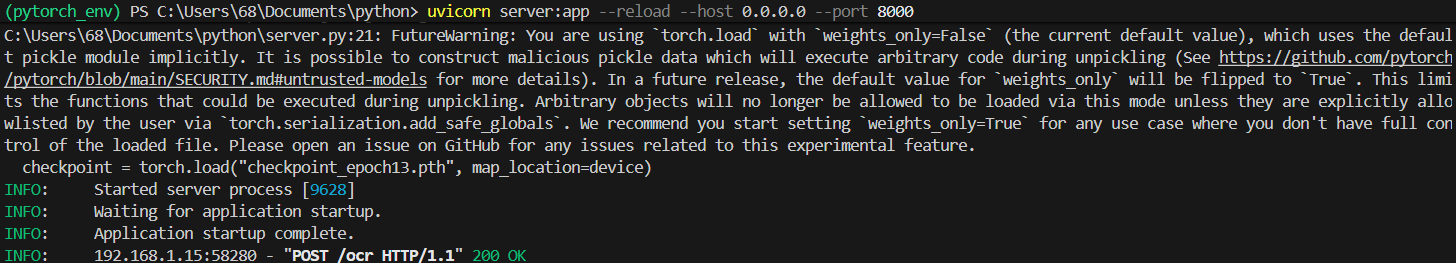
\includegraphics[width=0.85\textwidth]{Figures/whiletrain/pythonApi.png}
    \caption{OCR сургалтын backend Python API–ийн архитектурын диаграмм.}
    \label{fig:python-api}
  \end{figure}
}

%==============================================================================
% END OF FIGURE DEFINITIONS
%==============================================================================
